\documentclass[review, authoryear, 12pt]{elsarticle}

\usepackage{amssymb, amsmath}
\usepackage{amsfonts, bm, amssymb}
\usepackage{textcomp} % corresponding author
\usepackage{caption}
\captionsetup[figure]{labelfont=bf, labelsep=period, name={Fig.}}
\captionsetup[table]{labelfont=bf, labelsep=period, name={Table}}
\usepackage{subcaption}
\captionsetup[subfigure]{font=footnotesize}
\usepackage{booktabs} % three-line table
\usepackage{array} % table width setting
\usepackage{longtable} % across multiple pages
\usepackage{threeparttable} % table notes
\usepackage[hidelinks]{hyperref}
\usepackage{lineno} % line number
\usepackage[letterpaper, top=1in, bottom=1in, left=1in, right=1in]{geometry}
\usepackage{changes}
\usepackage{float}
\usepackage{xcolor}
\usepackage{etoolbox}

%% Article information for the accepted manuscript (placed between affiliations and abstract)
\definecolor{infoblue}{RGB}{0,112,192}
\newcommand{\articleinfo}{%
    \begin{minipage}{\textwidth}
    \normalsize\upshape\bfseries\raggedright\color{infoblue}\urlstyle{same}
    Article information: Zhang H, Wan B. Graph-based deep learning for compressive behavior of 3D-printed concrete columns across layers. Advances in Structural Engineering, 2026.\par\vskip6pt
    Link: \url{https://journals.sagepub.com/doi/10.1177/13694332261491070}\par\vskip6pt
    doi: \href{https://doi.org/10.1177/13694332261491070}{10.1177/13694332261491070}
    \end{minipage}}
\makeatletter
\patchcmd{\pprintMaketitle}{\hrule\vskip12pt}{\articleinfo\par\vskip24pt\hrule\vskip12pt}{}{\PackageWarning{manuscript}{Could not insert article information}}
\patchcmd{\MaketitleBox}{\hrule\vskip12pt}{\articleinfo\par\vskip24pt\hrule\vskip12pt}{}{\PackageWarning{manuscript}{Could not insert article information}}
\makeatother

\graphicspath{{figures/}}

\journal{Advances in Structural Engineering}

\begin{document}

\begin{frontmatter}

\title{Graph-Based Deep Learning for Compressive Behavior of 3D-Printed Concrete Columns across Layers} %% Article title

\author[mu]{Haoyou Zhang} %% Author name
\author[mu]{Baolin Wan\corref{cor1}} %% Author name
\ead{baolin.wan@marquette.edu}
\cortext[cor1]{Corresponding author}

%% Author affiliation
\affiliation[mu]{organization={Department of Civil, Construction, and Environmental Engineering, Marquette University},%Department and Organization
            addressline={1637 W. Wisconsin Ave.}, 
            city={Milwaukee},
            postcode={53201}, 
            state={WI},
            country={United States of America}}

\begin{abstract}
Extrusion-based three-dimensional concrete printing enables automated, formwork-free fabrication, but anisotropy and weak interlayer bonding complicate reliable prediction of the mechanical behavior of 3D-printed concrete (3DPC). This study developed a framework employing two parallel approaches, the finite element method (FEM) and physics-informed neural networks (PINNs), to simulate the compressive response of 3DPC. An open-source FEM formulation incorporating node-to-surface contact mechanics and the Mazars damage model was first established and validated against an experimentally tested 3DPC column, yielding a 19.5\% underestimation of load capacity and displacement errors within 7.7\%. PINNs were then adopted to embed governing mechanical laws directly into learning, improving physical consistency and interpretability over purely data-driven prediction. Two architectures, a multilayer perceptron (MLP) and a novel residual graph neural network (GNN), were evaluated against the FEM results. The GNN achieved a lower displacement root mean square error of $0.002\,\text{mm}$ than the MLP ($0.003\,\text{mm}$) while requiring fewer trainable parameters (90 vs. 141). Benign generalization analysis indicated that graph convolution reduced the required signal-to-noise ratio by approximately $1.4\times$, thereby enabling the model to extract the true signal in the presence of greater noise. Explainability analyses further showed that the $z$-coordinate dominated compressive-response prediction, while tangential coordinates governed interlayer behavior, and subgraph visualization revealed physically consistent stress and deformation pathways. The results show that coupling physics constraints with graph learning enhances both accuracy and interpretability, providing a pathway toward reliable structural design in 3DPC construction.

\vspace{1\baselineskip}
\end{abstract}

%Graphical abstract
\begin{graphicalabstract}
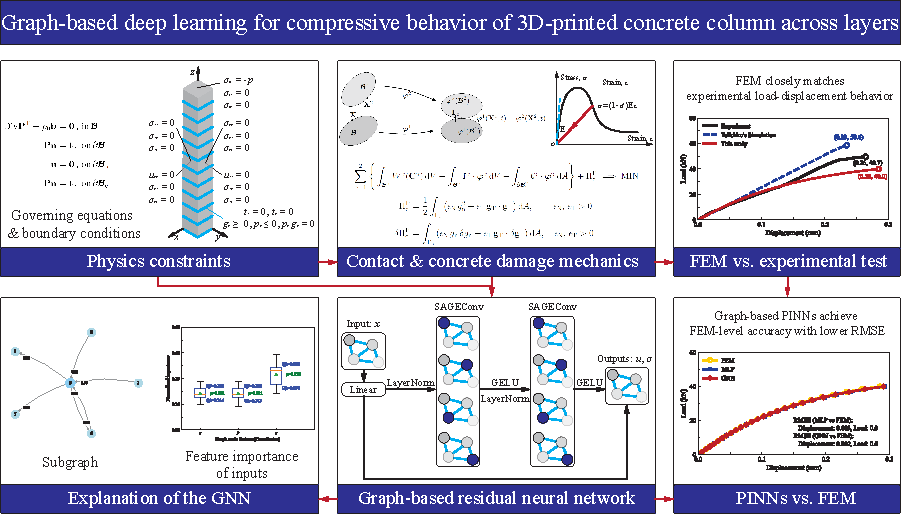
\includegraphics{graphical_abstract.pdf}
\end{graphicalabstract}

%Research highlights
\begin{highlights}
    \item Nonlinear 3DPC behavior is modeled through node-to-surface contact and Mazars damage.
    \item The residual GNN reproduces FEM displacement responses with an RMSE of 0.002 mm.
    \item The residual GNN matches MLP accuracy with only 90 trainable parameters versus 141.
    \item Benign generalization and explainability support noise robustness and physically meaningful learning.
\end{highlights}

%% Keywords
\begin{keyword}
Three-dimensional printed concrete; Contact mechanics; Finite element method; Physics-informed neural networks; Graph neural networks; Deep learning

\end{keyword}

\end{frontmatter}

\section*{Nomenclature}
\addcontentsline{toc}{section}{Notation} % adds to TOC if needed

\begin{longtable}{@{}ll@{}}

    \multicolumn{2}{@{}l}{\textbf{Contact mechanics}} \\[3pt]

    $g_{\text{n}}$ & Normal gap between active contact nodes \\
    $g_{\text{T} \alpha}$ ($\alpha = 1, \, 2$) & Tangential gap components between active contact nodes \\
    $n_{\text{c}}$ & Number of active contact nodes \\
    $p_{\text{n}}$ & Normal contact stress between active contact nodes \\
    $t_x$, $t_y$ & Tangential tractions in $x$ and $y$ directions on contact surface \\
    $A_s$ & Quadrature weight or area associated with the $s$-th contact point \\
    $C_{\text{c}}$ & Work contribution from active contact constraints \\
    $C_{\text{c}}^{\text{P}}$ & Work contribution from active contact constraints (penalty method) \\
    $C_{\text{c}}^{\text{st}}$ & Work contribution from active stick contact constraints \\
    $\epsilon$ & Penalty parameter \\
    $\epsilon_{\text{N}}$, $\epsilon_{\text{T}}$ & Penalty parameters in normal and tangential directions \\
    $\bm{\eta}_s$ & Virtual displacements for active stick contact constraints \\
    $\bar{\xi}^{\alpha}$ ($\alpha = 1, \, 2$) & Parametric coordinates \\
    $\bm{\xi}_0$ & Fixed parametric coordinates on the master surface (initial configuration) \\
    $\bm{\xi}_n$ & Parametric coordinates on the master surface at time $t = n$ \\
    $\bm{\Gamma}_{\text{c}}$ & Potential contact surface \\
    $\Pi_{\text{c}}^{\text{P}}$ & Penalty contact potential energy \\
    $\bar{\mathbf{a}}_{\alpha}$ ($\alpha = 1, \, 2$) & Surface tangential unit vectors \\
    $\mathbf{g}_s$ & Total stick gap vector from active stick contact constraints \\
    $\mathbf{g}_{\text{T}}$ & Tangential gap vector from active contact constraints \\
    $\mathbf{n}^1$ & Surface unit normal vector \\
    $\mathbf{t}$ & Prescribed traction on the contact boundary \\
    $\mathbf{u}_s$ & Displacement vector in the stick condition \\
    $\bar{\mathbf{x}}^1$ & Closest projection point on the master surface \\
    $\mathbf{B}_s$ & Traction transfer matrix in stick condition \\
    $\mathbf{G}_s^{\text{st}}$ & Internal force in stick condition \\
    $\mathbf{K}_s^{\text{st}}$ & Stick contact stiffness matrix (penalty method) \\
    $\partial \bm{\mathcal{B}}_{\text{c}}$ & Potential contact surface \\[6pt]


\multicolumn{2}{@{}l}{\textbf{Continuum mechanics, loading, and boundary conditions}} \\[3pt]

    $p$ & Applied compressive pressure on the column (positive) \\
    $t$ & Time \\
    $u_{xx}$, $u_{yy}$, $u_{zz}$ & Normal displacements on the $x$-, $y$- and $z$-faces \\
    $u_{xy}$, $u_{xz}$ & Shear displacements on the $x$-face in $y$ and $z$ directions \\
    $u_{yx}$, $u_{yz}$ & Shear displacements on the $y$-face in $x$ and $z$ directions \\
    $u_{zx}$, $u_{zy}$ & Shear displacements on the $z$-face in $x$ and $y$ directions \\
    $A$, $V$ & Surface area and volume of the body \\
    $\bm{\eta}^{\gamma}$ & Virtual displacement (test function) \\
    $\rho_0$ & Material density in the reference configuration \\
    $\sigma_{xx}$, $\sigma_{yy}$, $\sigma_{zz}$ & Normal stresses on the $x$-, $y$- and $z$-faces \\
    $\sigma_{xy}$, $\sigma_{xz}$ & Shear stresses on the $x$-face in $y$ and $z$ directions \\
    $\sigma_{yx}$, $\sigma_{yz}$ & Shear stresses on the $y$-face in $x$ and $z$ directions \\
    $\sigma_{zx}$, $\sigma_{zy}$ & Shear stresses on the $z$-face in $x$ and $y$ directions \\
    $\bm{\sigma}$, $\bm{\tau}$ & Cauchy stress tensor (second-order) and Kirchhoff stress tensor \\
    $\Pi$ & Total potential energy \\
    $\mathbf{b}$ & Body force in the reference configuration \\
    $\mathbf{f}^{\gamma}$ ($\gamma = 1, \, 2$) & Body force per unit volume in the reference configuration \\
    $\bar{\mathbf{t}}$ & Prescribed traction on non-contact boundaries \\
    $\mathbf{u}$ & Displacement vector \\
    $\mathbf{x}^{\alpha}$ ($\alpha = 1, \, 2$) & Spatial point in the body $\bm{\mathcal{B}}^{\alpha}$ \\
    $\mathbf{C}^{\gamma}$ & Right Cauchy-Green deformation tensor \\
    $\mathbf{F}^{\gamma}$ & Deformation gradient \\
    $\mathbf{P}$ & First Piola-Kirchhoff stress tensor \\
    $\bm{\mathcal{B}}^{\alpha}$ ($\alpha = 1, \, 2$) & Body configuration \\
    $\partial \bm{\mathcal{B}}$ & Boundary of the body \\
    $\partial\mathcal{B}_{\mathrm{t}}$,
    $\partial\mathcal{B}_{\mathrm{u}}$,
    & Traction and displacement portions of $\partial\mathcal{B}$ \\
    $\mathbf{X}^{\alpha}$ ($\alpha = 1, \, 2$) & Material point in the body $\bm{\mathcal{B}}^{\alpha}$ \\[6pt]


\multicolumn{2}{@{}l}{\textbf{Concrete damage model and material parameters}} \\[3pt]

    $d$ & Scalar damage variable \\
    $d_{\text{c}}$, $d_{\text{t}}$ & Uniaxial compressive and tensile damage variables \\
    $i_{\text{b}}$ & Tensile brittleness index (dimensionless) \\
    $A_{\text{c}}$, $A_{\text{t}}$ & Mazars model shape parameters in compression and tension \\
    $B_{\text{c}}$, $B_{\text{t}}$ & Mazars model damage evolution parameters in compression and tension \\
    $E$ & Scalar elastic modulus \\
    $\alpha_{\text{c}}$, $\alpha_{\text{t}}$ & Weights of uniaxial compressive and tensile damage \\
    $\epsilon_0$ & Strain threshold at the onset of damage \\
    $\epsilon_i$ ($i = 1, \, 2, \, 3$) & Principal strains \\
    $\epsilon_{\text{eq}}$ & von Mises equivalent strain \\
    $\epsilon_{\text{c}i}$, $\epsilon_{\text{t}i}$ ($i = 1, \, 2, \, 3$) & Compressive and tensile components of principal strains \\
    $\tilde{\epsilon}$ & Equivalent strain \\
    $\bm{\epsilon}$ & Strain tensor (second-order) \\
    $\kappa$ & Maximum equivalent strain reached in the loading history \\
    $\nu'$ & Modified Poisson's ratio \\
    $\psi$ & Helmholtz free energy \\
    $\mathbb{D}$ & Damage tensor (fourth-order) \\
    $\mathbb{E}$ & Elasticity tensor of undamaged concrete (fourth-order) \\[6pt]


\multicolumn{2}{@{}l}{\textbf{Graph/PINN and generalization quantities}} \\[3pt]

    $d_{\text{f}}$ & Dimension of the input feature vector \\
    $n_{\text{e}}$, $n_{\text{v}}$ & Number of edges and nodes in the graph \\
    $n_{\text{ts}}$ & Number of training samples \\
    $q$ & Exponent of the polynomial activation function \\
    $\text{r}_k$, $\text{s}_k$ & Receiver and sender nodes $k$ in the graph \\
    $x$ & Input to the neural network \\
    $C$ & Positive constant used in the SNR-based generalization bounds \\
    $D$ & Average node degree of the graph \\
    $\theta$ & Trainable parameters in the neural network \\
    $\theta^*$ & Optimized trainable parameters in the neural network \\
    $\boldsymbol{\mu}$ & Vector of true physics-based signal component in the input features \\
    $\sigma_{\text{p}}$ & Standard deviation (magnitude) of the noise component \\
    $\omega_{\mathcal{B}}$, $\omega_{\mathcal{D}}$, $\omega_{\mathcal{F}}$ & Weighted coefficients for boundary condition, labeled data and PDE losses \\
    $\mathbf{e}_k$, $\mathbf{v}_i$ & Edge $k$ and Node $i$ in the graph \\
    $\mathbf{E}$, $\mathbf{V}$ & Sets of edges and nodes in the graph \\
    $\bm{\mathcal{G}}$ & Graph matrix representation \\

\end{longtable}

\addtocounter{table}{-1}

\section{Introduction}
\label{introduction}

Extrusion-based three-dimensional concrete printing (3DCP) enables automated, cost-efficient, and formwork-free construction with reduced labor and material use~\citep{de_schutter_vision_2018, weng_comparative_2020, alshboul_advancing_2025}. Cementitious mortar is pumped through a nozzle and deposited layer by layer to form structures~\citep{paolini_additive_2019}. However, anisotropy, conflicting rheological requirements, and complex material-process-structure interactions remain major challenges, with mechanical performance being critical to structural safety and durability~\citep{lu_systematical_2019, shehadeh_advanced_2025}.

A key characteristic of hardened three-dimensional printed concrete (3DPC) is its anisotropic mechanical behavior caused by layer-wise construction~\citep{surehali_properties_2025}, as shown in Fig.~\ref{fig:printing_properties}. Compressive strengths in the $x$ and $y$ directions are generally similar but lower than that in the $z$ direction, mainly because weak interlayer interfaces promote shear failure under in-plane loading~\citep{joh_buildability_2020, zhang_evaluation_2024}. Therefore, understanding compression transfer across these interfaces is essential for the safe and efficient design of 3DPC structures~\citep{hassan_3d_2025}.

\begin{figure}[t]
    \centering
    \begin{subfigure}[t]{0.35\textwidth}
        \centering
        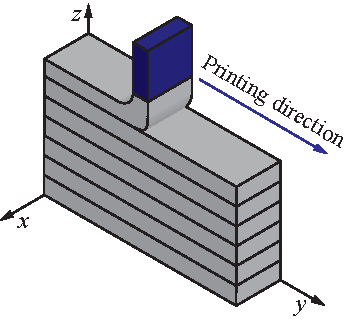
\includegraphics[width=0.75\textwidth]{printing_direction.pdf}
        \captionsetup{margin=-1em, justification=centering}
        \caption{Printing direction and layer stacking in extrusion-based 3DPC.}
    \end{subfigure}
    \kern 2em % Controls the exact gap between the two subfigure blocks
    \begin{subfigure}[t]{0.47\textwidth}
        \centering
        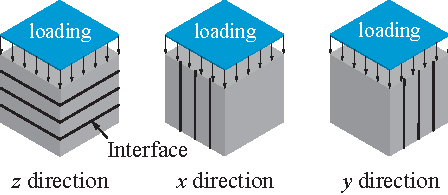
\includegraphics[width=0.9\textwidth]{loading_direction.pdf}
        \captionsetup{margin=-1em, justification=centering}
        \caption{Anisotropic mechanical response under loading along the $x$-, $y$-, and $z$-axes.}
    \end{subfigure}

    \caption{Layer stacking and anisotropic mechanical properties of 3DPC.}
    \label{fig:printing_properties}
\end{figure}

Interface-based models have been widely applied to capture the anisotropic behavior of 3DPC. \citet{xiao_finite_2021} modeled 3DPC beams in ABAQUS using concrete damaged plasticity for printed layers and cohesive elements for interfaces, achieving good agreement with flexural tests. To reduce computational cost, \citet{van_den_heever_mechanical_2021,van_den_heever_numerical_2022} developed two-dimensional DIANA models combining an anisotropic continuum formulation with an interface cracking-shearing-crushing model. For compression, \citet{tanapornraweekit_experimental_2022} simulated 3DPC walls in LS-DYNA using solid elements and Coulomb contact interfaces, while \citet{telichko_finite_2024} modeled a 3DPC column in ANSYS using solid elements and cohesive-zone interfaces. These studies demonstrate the capability of interface-based approaches to reproduce anisotropic and interlayer behavior, although accurate prediction of post-peak softening remains challenging. More recent studies have further examined the effects of porosity and interlayer properties~\citep{bayrak_3d_2024} and extended interface-based modeling to 3D-printed engineered cementitious composites~\citep{ye_size_2024}.

Machine learning (ML) has increasingly been applied to 3DCP, particularly for predicting the mechanical properties of hardened 3DPC~\citep{ali_machine_2023}. As summarized in Table~\ref{tab:summary_research}, most studies focus on compressive and flexural strength using methods such as artificial neural networks, random forests, support vector machines, and gradient-boosting algorithms~\citep{izadgoshasb_predicting_2021, ghasemi_tailoring_2023, uddin_novel_2024, zhu_eco-friendly_2024, zhang_research_2025, khodadadi_machine_2025}. Among these, ensemble methods such as XGBoost, LGBM, and GBR have generally shown strong predictive performance, with reported $R^2$ values often exceeding 0.9~\citep{ghasemi_tailoring_2023, uddin_novel_2024}. More recently, ML has also been extended beyond strength prediction to optimize mix design, pump speed, and carbon footprint~\citep{schossler_data-driven_2025}.

\begin{table}[!ht]
    \centering
    \footnotesize % \small
    \begin{threeparttable}
        \caption{Summary of ML studies on the mechanical properties of 3DPC.}
        \label{tab:summary_research}
        \setlength{\tabcolsep}{3pt}
        \begin{tabular}{
        >{\centering\arraybackslash}p{3.1cm}
        >{\centering\arraybackslash}p{4.3cm}
        >{\centering\arraybackslash}p{1.3cm}
        >{\centering\arraybackslash}p{0.6cm}
        >{\centering\arraybackslash}p{1.0cm}
        >{\centering\arraybackslash}p{1.6cm}
        >{\centering\arraybackslash}p{2.9cm}}
        \toprule
        Algorithms & Inputs & Outputs & TS & DS & Accuracy & Reference \\
        \midrule
        ANN & W/C, A, SP & CS & 65 & Exp. & $R = 0.98$ & \citet{izadgoshasb_predicting_2021} \\
        MR, XGBoost, RF & C, W, SP, SF, A, FA, age & CS & 307 & Exp. & $R^2 = 0.93$ & \citet{ghasemi_tailoring_2023} \\
        ANN, XGBoost, RF, GBR, LGBM, SVM, KNN, GEP & W/C, S/B, HM/B, SP/B, W/S, W/B, F, age, loading direction, D & CS & 299 & Exp. & $R^2 = 0.99$ & \citet{uddin_novel_2024} \\
        MR, SVM & S, rubber, epoxy, SF, F, D, dry and wet weight & CS, FS & 26 & Exp., num. & $R^2 = 0.94$ & \citet{zhu_eco-friendly_2024} \\
        MR, ANN, SVM, RF, DT & W/C, C, MA, A, admixture, F & CS, FS & 600 & Exp. & $R^2 = 0.98$ & \citet{zhang_research_2025} \\
        ANN & W/B, W, S, A, slag, HM, loading direction, F & FS & 127 & Exp. & $R^2 = 0.96$ & \citet{khodadadi_machine_2025} \\
        ANN, GBR, XGBoost, LGBM, AB, RF, DT & C, W, A, SF, SP, FA, slag, admixture, F & CS, PS, CF & 126 & Exp. & $R^2 = 0.99$ & \citet{schossler_data-driven_2025} \\
        \bottomrule
        \end{tabular}

        \begin{tablenotes}
        \footnotesize % \small
        \item \textbf{Note:}
        TS: number of training samples; DS: data source.

        ANN: artificial neural network; MR: multilinear regression; XGBoost: extreme gradient boosting; RF: random forest; GBR: gradient boosting regression; LGBM: light gradient boosting machine; SVM: support vector machine; KNN: $k$-nearest neighbors; GEP: gene expression programming; DT: decision tree; AB: adaptive boosting.

        W: water; C: cement; A: aggregate; SP: superplasticizer; FA: fly ash; SF: silica fume; F: fiber; D: dimension; S: sand; B: binder; HM: hydroxypropyl methylcellulose; MA: mineral admixture.

        CS: compressive strength; FS: flexural strength; PS: pump speed; CF: carbon footprint.

        Exp.: experimental; Num.: numerical.

        $R$: correlation coefficient; $R^2$: coefficient of determination.
        \end{tablenotes}
    \end{threeparttable}
\end{table}

Beyond material-property prediction, machine-learning methods have increasingly been adopted across civil and construction engineering to support automated coordination, design optimization, and risk-informed decision-making. A modified extreme gradient boosting model has been used to improve multidisciplinary clash detection in building information modeling~\citep{shehadeh_enhanced_2024}, while the integration of convolutional, graph, and recurrent neural networks with virtual-reality-enabled BIM has been explored for proactive clash identification and engineering design optimization~\citep{shehadeh_enhancing_2025}. In construction safety, advanced ensemble methods, including XGBoost, LightGBM, and a modified decision tree, have been applied to predict occupational injury risks and support targeted preventive interventions~\citep{shehadeh_enhancing_2025-1}. Collectively, these studies demonstrate the growing role of intelligent computational methods in construction. However, these applications remain predominantly data-driven, motivating physics-informed models that embed governing mechanical principles when predicting structural displacement and stress fields.

Physics-informed neural networks (PINNs) have gained attention for improving interpretability and reducing reliance on large labeled datasets. In 3DCP, PINNs have been applied to model the rheological behavior of fresh cementitious materials by embedding governing flow equations into training~\citep{zhang_rheologynet_2023, yan_physics-informed_2025, zhang_navierstokes-informed_2025}. They have also been explored to accelerate nonlinear finite element analysis~\citep{ekanayaka_modeling_2023}. More recently, physics-informed graph neural networks (GNNs) have been introduced to better represent complex 3D-printed geometries and structural responses~\citep{wang_physics-informed_2025}.

Despite growing interest in predicting the mechanical behavior of 3DPC, important limitations remain. Existing machine-learning models are predominantly data-driven and focus on peak strengths, with limited capability to resolve displacement and stress fields or provide physical interpretability. Numerical studies explicitly representing load transfer across multiple interlayer interfaces remain scarce, while conventional multilayer-perceptron-based PINNs treat spatial points independently and do not directly exploit structural connectivity. These gaps motivate the development of a physics-informed graph framework for multilayer 3DPC. Accordingly, this study aims to: (1) establish and experimentally validate an open-source finite element method (FEM) framework incorporating node-to-surface contact and concrete damage mechanics; (2) develop PINNs for predicting spatial displacement and stress fields under governing mechanical constraints; and (3) evaluate whether graph-based learning improves accuracy, parameter efficiency, robustness, and interpretability relative to a conventional multilayer perceptron (MLP).

The principal contributions are fourfold. First, the FEM formulation combines interlayer contact mechanics with the Mazars damage model to provide a transparent and reproducible representation of multilayer 3DPC under compression. Second, the PINN framework extends prediction from peak quantities to spatially resolved mechanical fields while enforcing equilibrium and boundary conditions. Third, a residual graph neural network is introduced to incorporate local spatial connectivity and achieve comparable or improved accuracy with fewer trainable parameters than the MLP. Fourth, benign generalization and graph-explainability analyses are used to examine noise robustness, influential spatial features, and message-passing pathways, providing theoretical and interpretable evidence for the graph-based formulation.

\section{Contact Mechanics-Based Finite Element Model with Concrete Damage}

\subsection{Node-to-Surface Contact Model for Interfaces}
\label{subsec:node_to_surface}

Contact problems are boundary-value problems in which governing equations apply within the bodies and contact constraints act along their interfaces~\citep{laursen_continuum-based_1993, wriggers_computational_2006}. The main discretization schemes are node-to-node, surface-to-surface, and node-to-surface contact, as shown in Fig.~\ref{fig:node_surface_contact}. Node-to-node methods require matching meshes and are unsuitable for large deformation or sliding~\citep{francavilla_note_1975, sun_novel_2023}. Surface-to-surface formulations are accurate but involve complex projections, higher computational cost, and additional stability requirements~\citep{wohlmuth_mortar_2000, el-abbasi_stability_2001, jin_node--node_2016}. By contrast, node-to-surface contact provides a robust and efficient alternative for non-matching meshes, large sliding, and evolving or irregular contact zones~\citep{bathe_solution_1985, sun_novel_2023, das_systematic_2024}.

\begin{figure}[t]
    \centering
    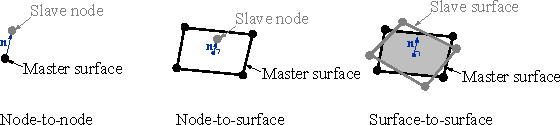
\includegraphics[width=0.8\textwidth]{node_surface_contact.pdf}
    \captionsetup{justification=centering}
    \caption{Comparison of contact discretization schemes.}
    \label{fig:node_surface_contact}
\end{figure}

\subsubsection{Contact Kinematics}

Fig.~\ref{fig:node_to_surface_coordinates} shows two bodies $\bm{\mathcal{B}}^{\alpha}$ ($\alpha = 1, \, 2$) in $\mathbb{E}^3$, whose configurations are defined by $\bm{\varphi}^{\alpha}: \bm{\mathcal{B}}^{\alpha} \to \mathbb{E}^3$, with $\mathbf{x}^{\alpha}=\bm{\varphi}^{\alpha}(\mathbf{X}^{\alpha})$. At contact, the gap is decomposed into the normal gap $g_{\text{n}}$, which measures separation or penetration, and the tangential gap $\mathbf{g}_{\text{T}}$, which describes relative sliding. The projection point $\bar{\mathbf{x}}^1$ and convective coordinates $(\bar{\xi}^1,\bar{\xi}^2)$ locate the slave point projection on the master surface. The normal gap is defined as
\begin{align}
    g_{\text{n}} = \left[ \mathbf{x}^2 - \mathbf{x}^1 \left( \bar{\xi}^1, \bar{\xi}^2 \right) \right] \cdot \mathbf{n}^1 \label{eq:g_N} %\,,
\end{align}
where $\mathbf{x}^2$ is the slave point; $\mathbf{x}^1(\bar{\xi}^1,\bar{\xi}^2)$ is its closest projection on the master surface; and $\mathbf{n}^1$ is the outward unit normal. The tangential gap vector is
\begin{align}
    \mathbf{g}_{\text{T}} = g_{\text{T} \alpha} \bar{\mathbf{a}}_{\alpha} = 0 \,, \quad g_{\text{T} \alpha} = (\mathbf{x}^2 - \bar{\mathbf{x}}^1) \cdot \bar{\mathbf{a}}_{\alpha}^1 % \,,
\end{align}
where $\bar{\mathbf{a}}_{\alpha} = \partial \mathbf{x}^{1} / \partial \xi^{\alpha}$ are the surface tangential basis vectors at the projection point.

\begin{figure}[t]
    \centering
    \begin{subfigure}{0.6\textwidth}
        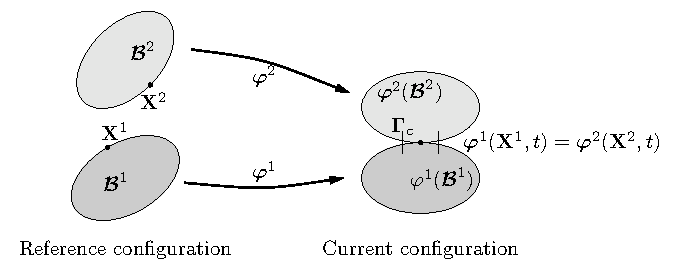
\includegraphics[width=\textwidth]{contact_kinematics_pdf.pdf}
        \caption{Finite deformation contact system between two bodies.}
    \end{subfigure}

    \vspace{0.5em}

    \centering
    \begin{subfigure}{0.55\textwidth}
        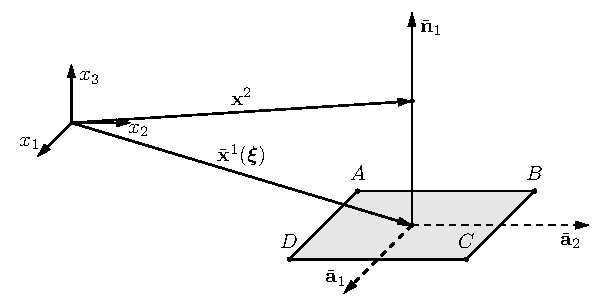
\includegraphics[width=\textwidth]{node_to_surface_coordinates_pdf.pdf}
        \captionsetup{margin={-4em, -4em}, justification=centering}
        \caption{Projection of the slave point onto the master surface and local coordinate system.}
    \end{subfigure}

    \caption{Finite deformation contact kinematics and node-to-surface projection for gap evaluation.}
    \label{fig:node_to_surface_coordinates}
\end{figure}


\subsubsection{Weak Form of Contact Conditions}

Consider a hyperelastic body $\bm{\mathcal{B}}$ in the reference configuration, subjected to body forces $\mathbf{b}$ and prescribed boundary tractions. Its boundary is decomposed as $\partial \bm{\mathcal{B}} = \partial \bm{\mathcal{B}}_{\text{t}} \cup \partial \bm{\mathcal{B}}_{\text{u}} \cup \partial \bm{\mathcal{B}}_{\text{c}}$, denoting the Neumann, Dirichlet, and potential contact surfaces, respectively. Under quasistatic conditions, equilibrium is governed by
\begin{align}
    \text{Div} \mathbf{P}^\text{T} + \rho_0 \mathbf{b} &= \mathbf{0} \,, &&\text{in} \, \bm{\mathcal{B}} \\ % \,;
    \mathbf{P} \mathbf{n} &= \bar{\mathbf{t}} \,, &&\text{on} \, \partial \bm{\mathcal{B}}_{\text{t}} \\ % \,;
    \mathbf{u} &= \mathbf{0} \,, &&\text{on} \, \partial \bm{\mathcal{B}}_{\text{u}} \\ % \,;
    \mathbf{P} \mathbf{n} &= \mathbf{t} \,, &&\text{on} \, \partial \bm{\mathcal{B}}_{\text{c}} %\,;
\end{align}
where $\mathbf{P}$ is the first Piola-Kirchhoff stress tensor; $\rho_0$ is the reference density; $\bar{\mathbf{t}}$ and $\mathbf{t}$ are prescribed tractions acting on the outward normal $\mathbf{n}$; and $\mathbf{u}$ is the displacement vector. For two deformable bodies, the weak form is
\begin{align}
    \sum_{\gamma=1}^2 \Bigg\{ 
        \int_{\bm{\mathcal{B}}^{\gamma}} \bm{\tau}^{\gamma} \cdot \text{grad} \, \bm{\eta}^{\gamma} \, \text{d}V 
        - \int_{\bm{\mathcal{B}}^{\gamma}} \mathbf{f}^{\gamma} \cdot \bm{\eta}^{\gamma} \, \text{d}V 
        - \int_{\partial \bm{\mathcal{B}}_{\text{t}}^{\gamma}} \bar{\mathbf{t}}^{\gamma} \cdot \bm{\eta}^{\gamma} \, \text{d}A 
        \Bigg\} 
    + C_{\text{c}} = 0 %\,,
\end{align}
where $\bm{\tau} = \mathbf{P}^{\gamma} \mathbf{F}^{\gamma \text{T}}$ is the Kirchhoff stress tensor; $\mathbf{F}^{\gamma} = \text{grad} \bm{\varphi}$ is the deformation gradient; $\mathbf{f}^{\gamma} = \rho_0^{\gamma} \mathbf{b}^{\gamma}$ is the body force per unit reference volume; and $\bm{\eta}^{\gamma} \in V$ is the virtual displacement vanishing on $\partial \bm{\mathcal{B}}_{\text{u}}^{\gamma}$. The term $C_{\text{c}}$ represents the active contact contribution.

The total potential energy represents the balance among the internal energy stored in the deformable bodies, the work performed by external body forces and prescribed tractions, and the energy associated with the contact constraints. The internal strain energy describes the elastic response of the material, while material degradation due to concrete damage is introduced separately through the damage-dependent constitutive formulation described in Section~\ref{subsec:concrete_damage}. The equilibrium configuration is obtained by minimizing
\begin{align}
    \sum_{\gamma=1}^2 \Bigg\{ 
        \int_{\bm{\mathcal{B}}^{\gamma}} W^{\gamma}(\mathbf{C}^{\gamma}) \, \text{d}V 
        - \int_{\bm{\mathcal{B}}^{\gamma}} \mathbf{f}^{\gamma} \cdot \bm{\varphi}^{\gamma} \, \text{d}V 
        - \int_{\partial \bm{\mathcal{B}}_{\text{t}}^{\gamma}} \bar{\mathbf{t}}^{\gamma} \cdot \bm{\varphi}^{\gamma} \, \text{d}A 
    \Bigg\} 
    + \Pi_{\text{c}}^{\text{P}} \implies \text{MIN} \label{eq:min_total_energy} % \,,
\end{align}
where $W^{\gamma}(\mathbf{C}^{\gamma})$ is the strain energy density expressed in terms of $\mathbf{C}^{\gamma} = \mathbf{F}^{\text{T}} \mathbf{F}$; $\bm{\varphi}^{\gamma}$ is the deformation mapping of $\bm{\mathcal{B}}^{\gamma}$; and $\Pi_{\text{c}}$ is the contact potential energy. The penalty formulations of $\Pi_{\text{c}}$ and $C_{\text{c}}$ are introduced in the following section.

\subsubsection{Penalty Method for Contact Constraints}
\label{subsubsec:penalty_method}

The penalty method enforces contact constraints through a spring-like force proportional to surface penetration. It is straightforward to implement and introduces no additional unknowns. However, the penalty parameter must be selected carefully: low values permit excessive penetration, whereas high values may cause ill-conditioning, numerical instability, and convergence difficulties.

A penalty term is added to the total potential energy $\Pi$ in Eqn.~(\ref{eq:min_total_energy}):
\begin{align}
    \Pi_{\text{c}}^{\text{P}} = \frac{1}{2} \int_{\partial \bm{\mathcal{B}}_{\text{c}}} 
    \left( 
        \epsilon_{\text{N}} \, g_{\text{n}}^2 + \epsilon_{\text{T}} \, \mathbf{g}_{\text{T}} \cdot \mathbf{g}_{\text{T}} 
    \right) \text{d}A, 
    \quad \epsilon_{\text{N}}, \, \epsilon_{\text{T}} > 0 \label{eq:Pi_cPenalty} % \,,
\end{align}
where $\epsilon_{\text{N}}$ and $\epsilon_{\text{T}}$ are the normal and tangential penalty parameters, respectively. Its variation yields the contact contribution to the weak form:
\begin{align}
    C_{\text{c}}^{\text{P}} = \delta \Pi_{\text{c}}^{\text{P}} = \int_{\partial \bm{\mathcal{B}}_{\text{c}}} 
    \left( 
    \epsilon_{\text{N}} \, g_{\text{n}} \, \delta g_{\text{n}} + \epsilon_{\text{T}} \, \mathbf{g}_{\text{T}} \cdot \delta \mathbf{g}_{\text{T}} 
    \right) \text{d}A, 
    \quad \epsilon_{\text{N}}, \, \epsilon_{\text{T}} > 0  \label{eq:varation_Pi_cPenalty} %\,.
\end{align}
In the stick regime, the projection coordinates remain fixed, and the stick gap is
\begin{align}
    \mathbf{g}_s = \mathbf{x}^2 - \mathbf{x}^1(\bm{\xi}_0) \,,
        \quad \delta \mathbf{g}_s = \bm{\eta}^2 - \bm{\eta}^1(\bm{\xi}_0)
\end{align}
which gives the discrete contact contribution
\begin{align}
    C_{\text{c}}^{\text{st}} = \int_{\partial \bm{\mathcal{B}}_{\text{c}}} \mathbf{t} \cdot \delta \mathbf{g}_s \, \text{d}A
        = \sum_{s=1}^{n_{\text{c}}} A_s \bm{\eta}_s^{\text{T}} \mathbf{G}_s^{\text{st}} \,, \quad
        \mathbf{G}_s^{\text{st}} = \mathbf{B}_{\text{s}} \, \mathbf{t} \,,
\end{align}
\begin{align}
    \mathbf{B}_s = 
    \begin{bmatrix}
        \mathbf{1} &
        -N_1(\bm{\xi}_0) \, \mathbf{1} &
        -N_2(\bm{\xi}_0) \, \mathbf{1} &
        -N_3(\bm{\xi}_0) \, \mathbf{1} &
        -N_4(\bm{\xi}_0) \, \mathbf{1}
    \end{bmatrix}^{\mathrm{T}} %\, ,
\end{align}
where $\bm{\xi}_0$ denotes the fixed master-surface coordinates; $n_{\text{c}}$ is the number of active contact nodes, $A_s$ is the quadrature weight or associated area; $\bm{\eta}_s^{\text{T}}$ collects the virtual displacements of the slave and master nodes; and $\mathbf{G}_s^{\text{st}}$ is the stick internal-force contribution. The matrix $\mathbf{1}$ is the $3 \times 3$ identity matrix, and $N_i(\bm{\xi}_0)$ are the master-element shape functions evaluated at $\bm{\xi}_0$. Because $\bm{\xi}_0$ remains fixed during sticking, linearization gives
\begin{align}
    \Delta C_{\text{c}}^{\text{st}} = \sum_{s=1}^{n_{\text{c}}} A_s \bm{\eta}_s^{\text{T}} \Delta \mathbf{G}_s^{\text{st}}
    = \sum_{s=1}^{n_{\text{c}}} A_s \bm{\eta}_s^{\text{T}} \mathbf{K}_s^{\text{st}} \Delta \mathbf{u}_s %\, ,
\end{align}
with
\begin{align}
    \mathbf{K}_s^{\text{st}} = \epsilon \, \mathbf{B}_s \mathbf{B}_s^{\text{T}} % \,.
\end{align}
Here, $\mathbf{K}_s^{\text{st}}$ is the incremental stiffness enforcing the stick constraint, while $\mathbf{B}_s$ distributes the contact interaction between the slave node and the master-surface nodes through the shape functions.

\subsection{Concrete Damage Model for Nonlinearity}
\label{subsec:concrete_damage}

\subsubsection{Fundamentals of Elastic Damage Model}

Concrete damage is irreversible and must satisfy thermodynamic principles. Under isothermal conditions, admissible constitutive behavior is governed by the Clausius-Duhem inequality,
\begin{align}
    \left( \bm{\sigma} - \frac{\partial \psi}{\partial \bm{\epsilon}} \right) \dot{\bm{\epsilon}} - \frac{\partial \psi}{\partial \mathbb{D}} \dot{\mathbb{D}} \geq 0 %\,,
\end{align}
where $\bm{\sigma} = \sigma_{ij}$ is the second-order Cauchy stress tensor; $\psi$ is the Helmholtz free energy dependent on $\bm{\epsilon}$ and $\mathbb{D}$; $\bm{\epsilon} = \epsilon_{ij}$ is the second-order strain tensor; and $\mathbb{D} = D_{ijkl}$ is the fourth-order damage tensor. Thermodynamic consistency requires
\begin{align}
    \bm{\sigma} = \frac{\partial \psi}{\partial \bm{\epsilon}} \,, \quad
    -\frac{\partial \psi}{\partial \mathbb{D}} \dot{\mathbb{D}} \geq 0
\end{align}
which define the damaged stress-strain relation and ensure dissipative damage evolution, forming the basis of elastic damage models for concrete.

\subsubsection{Original Mazars Damage Model}

To represent post-elastic stiffness degradation, the original Mazars damage model~\citep{mazars_continuum_1989} is adopted. This scalar isotropic formulation reduces elastic stiffness through a damage variable and captures tension-compression asymmetry using separate tensile and compressive contributions. Concrete degradation within printed layers is modeled by Mazars damage, while interlayer discontinuities and load transfer are represented by node-to-surface contact.

Before damage initiation ($d = 0$), concrete is linearly elastic, while the damaged constitutive relation is
\begin{align}
    \bm{\sigma} = (1 - d) \mathbb{E} \bm{\epsilon} %\,,
\end{align}
where $d \in [0, \, 1]$ is the scalar damage variable and $\mathbb{E} = E_{ijkl}$ is the fourth-order elasticity tensor of undamaged concrete, as illustrated in Fig.~\ref{fig:mazars_damage}. Tension-compression asymmetry is represented by
\begin{align}
    d = \alpha_{\text{t}} d_{\text{t}} + \alpha_{\text{c}} d_{\text{c}}, \quad \text{with} \, \alpha_{\text{t}} + \alpha_{\text{c}} = 1 %\,.
\end{align}
where the weighting coefficients are determined from the principal strains:
\begin{align}
    \alpha_{\text{t}} = \frac{\langle \epsilon_{\text{t}i} \rangle \epsilon_{\text{t}i}}{\tilde{\epsilon}^{2}}, \quad \alpha_{\text{c}} = \frac{\langle \epsilon_{\text{c}i} \rangle \epsilon_{\text{c}i}}{\tilde{\epsilon}^{2}} %\,.
\end{align}
The principal strains $\epsilon_i$ ($i = 1, \, 2, \, 3$) are decomposed as $\epsilon_i = \epsilon_{\text{t}i} + \epsilon_{\text{c}i}$. The Macaulay brackets $\langle \epsilon_{i} \rangle = \text{max} (\epsilon_i, \, 0)$ retain the tensile components, and the equivalent strain is
\begin{align}
    \tilde{\epsilon} = \sqrt{\langle \epsilon_{i} \rangle \langle \epsilon_{i} \rangle} %\,.
\end{align}
The tensile and compressive damage variables evolve independently:
\begin{align}
    d_{\text{t}} = 1 - \frac{(1 - A_{\text{t}})\epsilon_{0}}{\kappa} - A_{\text{t}} e^{-B_{\text{t}}(\kappa - \epsilon_{0})} %\,,
\end{align}
\begin{align}
    d_{\text{c}} = 1 - \frac{(1 - A_{\text{c}})\epsilon_{0}}{\kappa} - A_{\text{c}} e^{-B_{\text{c}}(\kappa - \epsilon_{0})} %\,,
\end{align}
where $A_{\text{t}}, \, B_{\text{t}}, \, A_{\text{c}}, \, B_{\text{c}}$ govern the post-peak response and are calibrated from uniaxial tests. Here, $\epsilon_0$ is the damage-initiation strain, and $\kappa = \text{max} (\tilde{\epsilon}, \, \epsilon_0)$ is the maximum equivalent strain attained during loading.

\begin{figure}[t]
    \centering
    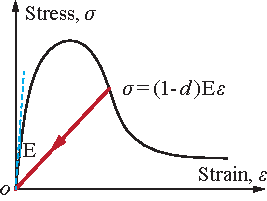
\includegraphics[width=0.25\textwidth]{mazars_damage.pdf}
    \caption{Constitutive law of the original Mazars damage model.}
    \label{fig:mazars_damage}
\end{figure}

\section{Physics-Informed Graph Neural Network Model}

\subsection{Physics-Informed Neural Networks}

PINNs embed governing differential equations and boundary/initial conditions directly into the neural network loss function, enabling physics-constrained solution learning~\citep{jin_recent_2023, haghighat_physics-informed_2021}. The solution $u(x)$ is approximated by a neural network $\hat{u}_{\theta}(x)$ with trainable parameters $\theta$:
\begin{align}
    \hat{u}_{\theta}(x) \approx u(x) %\,,
    \label{eq:pinn_general_formula}
\end{align}
Training minimizes a composite loss comprising the governing-equation residual $\mathcal{L}_{\mathcal{F}}$, boundary conditions $\mathcal{L}_{\mathcal{B}}$, and, when available, labeled data $\mathcal{L}_{data}$:
\begin{align}
    \theta^* = \arg \min_{\theta} \left( \omega_{\mathcal{F}} \mathcal{L}_{\mathcal{F}}(\theta) + \omega_{\mathcal{B}} \mathcal{L}_{\mathcal{B}}(\theta) + \omega_{\mathcal{D}} \mathcal{L}_{data}(\theta) \right) % \,.
    \label{eq:general_nn}
\end{align}
In this study, the governing equation is:
\begin{align}
    \bm{\nabla} \cdot \bm{\sigma} + \mathbf{b} = \mathbf{0} \, \quad \text{in} \, \bm{\mathcal{B}}
    \label{eq:governing_equation}
\end{align}
where $\mathbf{b} = \mathbf{0}$. The boundary conditions are given in Section~\ref{subsec:iterative_framework}. No labeled data are used; therefore, training is fully unsupervised, with all loss-term weights set to 1.0.

Using automatic differentiation (AD), PINNs compute derivatives without conventional discretization or meshes and can approximate complex functions efficiently~\citep{grossmann_can_2024}. As shown in Fig.~\ref{fig:pinn}, a PINN consists of three components: (1) a neural network mapping input variables $x$ to the approximate solution $u$; (2) a physics-informed component using AD to enforce governing equations (GEs) and boundary/initial conditions (BCs/ICs); and (3) an optimization loop that minimizes the total loss and updates the trainable parameters $\theta$.

\begin{figure}[t]
    \centering
    \begin{minipage}[t]{0.48\textwidth}
        \centering
        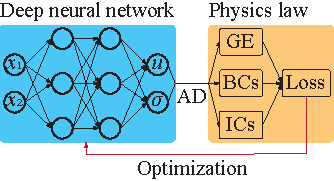
\includegraphics[width=0.65\textwidth]{pinn.pdf}
        \caption{General physics-informed neural network.}
        \label{fig:pinn}
    \end{minipage}
    \hfill % Explicit horizontal space between the two figures
    \begin{minipage}[t]{0.47\textwidth}
        \centering
        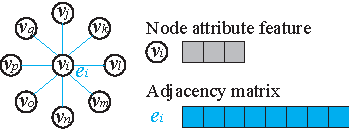
\includegraphics[width=0.8\textwidth]{graph.pdf}
        \caption{Graph network elements and connectivity.}
        \label{fig:graph}
    \end{minipage}
\end{figure}

\subsection{Graph Representation and Graph Convolution}

Graphs, denoted as $\bm{\mathcal{G}} = (\mathbf{V}, \mathbf{E})$, represent interactions among discrete entities~\citep{feng_energy-informed_2024}. As shown in Fig.~\ref{fig:graph}, $\mathbf{V}$ and $\mathbf{E}$ denote the node and edge sets, respectively. Each node $\mathbf{v}_i \in \mathbf{V}$ carries an attribute vector, while each edge $\mathbf{e}_k \in \mathbf{E}$ represents a directed connection from sender $\mathbf{v}_{\text{s}_k}$ to receiver $\mathbf{v}_{\text{r}_k}$. The node set is $\mathbf{V} = \{ \mathbf{v}_i \}_{i=1}^{n_{\text{v}}}$, where $n_{\text{v}}$ is the number of nodes, and the neighborhood of $\mathbf{v}_1$ is $\mathcal{N}(\mathbf{v}_1) = \{ \mathbf{v}_2 \in \mathbf{V} \mid (\mathbf{v}_1, \mathbf{v}_2) \in \mathbf{E} \}$. The edge set is $\mathbf{E} = \{ (\mathbf{e}_k, \mathbf{v}_{\text{r}_k}, \mathbf{v}_{\text{s}_k}) \}_{k=1}^{n_{\text{e}}}$, where $n_{\text{e}}$ is the number of edges and $\text{r}_k$ and $\text{s}_k$ identify the receiver and sender nodes.

In this study, each node represents a normalized spatial collocation point in the PINN domain rather than an FEM mesh node, and its attribute vector contains the $x$-, $y$-, and $z$-coordinates. Each node is connected to its eight nearest spatial neighbors, while no explicit edge attributes are used. Boundary points are identified from their coordinates, and the governing equilibrium, displacement, traction, and contact conditions are imposed through the physics-informed loss. The geometry and material properties are fixed prescribed parameters rather than node or edge features. The GNN predicts three displacement and six stress components at each node.

Graph convolutional networks (GCNs)~\citep{kipf_semi-supervised_2017} extend convolution to graph-structured data by aggregating neighboring-node features, followed by linear transformation and nonlinear activation. Building on this principle, GraphSAGE (SAmple and aggreGatE)~\citep{hamilton_inductive_2017} samples a fixed number of neighbors (eight in this study) and aggregates their features using learned functions such as mean or pooling. As shown in Fig.~\ref{fig:GraphSAGE}, this neighborhood-sampling and aggregation process enables scalable, permutation-invariant learning and generalization to unseen nodes and graphs~\citep{wu_comprehensive_2021, georgousis_graph_2021}.

\begin{figure}[t]
    \centering
    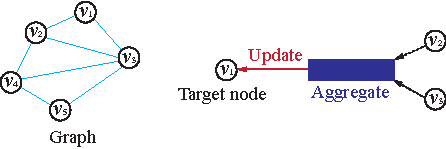
\includegraphics[width=0.5\textwidth]{GraphSAGE.pdf}
    \caption{Schematic illustration of the GraphSAGE framework.}
    \label{fig:GraphSAGE}
\end{figure}

\section{Validation of Finite Element Model with Experimental Test}
\subsection{Specimen Configuration and Numerical Modeling}

A numerical simulation was conducted on an eleven-layer 3DPC column based on the experiment by~\citet{telichko_finite_2024}, as shown in Fig.~\ref{fig:compression_across_layers}. The specimen has a $40 \, \text{mm} \times 40 \, \text{mm}$ cross-section, a total height of $165 \, \text{mm}$, and ten interlayer interfaces formed by $15 \, \text{mm}$-high layers. The printing path follows the $x$-axis, while compression is applied perpendicular to the interfaces. Material properties are listed in Table~\ref{tab:material_parameters}. Due to limited tensile data, the material is assumed linear elastic up to the tensile strength, with the same elastic modulus used in tension and compression.

\begin{figure}[t]
    \centering
    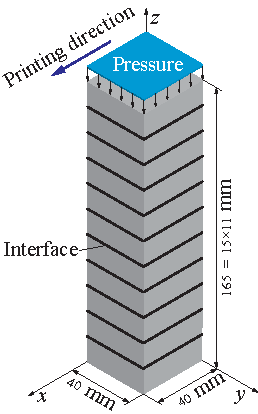
\includegraphics[width=0.25\textwidth]{column.pdf}
    \captionsetup{justification=centering}
    \caption{Eleven-layer 3DPC column under perpendicular compressive loading~\citep{telichko_finite_2024}.}
    \label{fig:compression_across_layers}
\end{figure}

\begin{table}[t]
    \centering
    \footnotesize
    \caption{Material parameters used in the finite element model~\citep{telichko_finite_2024}.}
    \label{tab:material_parameters}
    \begin{tabular}{lcc}
        \toprule
        Parameter & Symbol & Value \\
        \midrule
        Elastic modulus & $ \text{E} $ & $ 26.5 \, \text{GPa} $ \\
        Poisson's ratio & $ \nu $ & $ 0.25 $ \\
        Uniaxial compressive strength & $ f_\text{c} $ & $ 50.3 \, \text{MPa} $ \\
        Uniaxial tensile strength & $ f_\text{t} $ & $ 1.29 \, \text{MPa} $ \\
        \bottomrule
    \end{tabular}
\end{table}

The node-to-surface formulation is used to model the interlayer interfaces. Following Section~\ref{subsubsec:penalty_method}, the normal and tangential penalty stiffnesses are both set to $1 \times 10^{12} \, \text{N/mm}$ based on~\citet{laursen_continuum-based_1993}, providing strong contact enforcement without excessive numerical instability. Material degradation is represented by the original Mazars model with $A_\text{c} = A_\text{t} = 1.0$, $B_\text{c} = 3000$, and $B_\text{t} = 41{,}085$~\citep{mazars_using_2006, mazars_new_2015, mazars_damage_2022}. The tensile parameter $B_\text{t}$ is calculated following~\citet{debuisne_need_2024}:
\begin{align}
    B_\text{t} = \frac{1 + i_{\text{b}}}{\epsilon_0} %,
\end{align}
where $i_{\text{b}}$ is the tensile brittleness index, taken as $1.0$ in this study; and $\epsilon_0$ is the damage initiation strain.

\subsection{Load--Displacement Response and Failure Analysis}

The load-displacement response under load-controlled compression is shown in Fig.~\ref{fig:load_disp_across_layers}. The experimental uniaxial compressive strength reported by~\citet{telichko_finite_2024} corresponded to a peak load of $49.7 \, \text{kN}$ at a displacement of $0.26 \, \text{mm}$. Their numerical simulation using ANSYS predicted a maximum load of $58.6 \, \text{kN}$ at $0.23 \, \text{mm}$, yielding load and displacement errors of approximately $17.9\%$ and $-11.5\%$, respectively. The limited nonlinearity in Telichko's simulation may be attributed to relatively large default penalty parameters in ANSYS, which likely enforced overly stiff interfacial bonds, suppressing interface degradation and damage evolution. In contrast, the present simulation predicted a peak load of $40.0 \, \text{kN}$ at a displacement of $0.28 \, \text{mm}$. The predicted response agrees well with the experimental results, particularly for displacements below $0.15 \, \text{mm}$. Beyond this peak, the maximum Mazars concrete damage $d$ exceeded $0.8$, indicating that the residual strength of concrete had fallen below $20\%$, a threshold typically regarded as failure~\citep{fema_356_2000, asce_41_2023}. After peak loading, the load plateaued with only slight increases while displacement continued to grow rapidly, eventually leading to numerical instability due to large deformations. These results signal that the load-bearing capacity had been reached. The corresponding load and displacement errors were approximately $-19.5\%$ and $7.7\%$, respectively. These results capture the concrete behavior well for displacements below $0.15 \, \text{mm}$, corresponding to a total strain of 0.001. However, the simulated strength is lower than the experimental value because, at a displacement of $0.15 \, \text{mm}$, the load has already reached roughly $30 \, \text{kN}$, which is 60\% of the peak load. This indicates that the material has entered the nonlinear regime, where concrete behavior becomes significantly more difficult to model accurately~\citep{hsu_fatigue_1984, wee_stress-strain_1996}. At this stage, the Mazars damage model experiences rapid damage evolution, a known issue associated with non-regularized damage formulations. Such models are prone to strain localization, which can accelerate stiffness degradation and lead to underestimation of strength~\citep{lemaitre_course_2013, arruda_modified_2022, legeron_damage_2005}.

\begin{figure}[t]
    \centering
    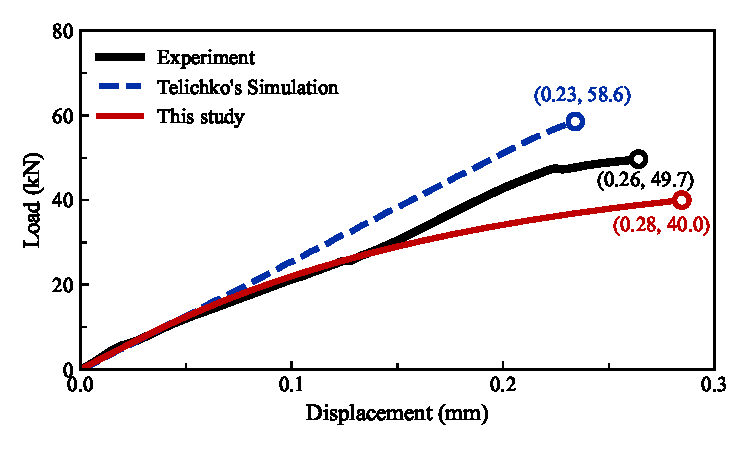
\includegraphics[width=0.65\textwidth]{Load_disp_across_layers.pdf}
    \captionsetup{justification=centering}
    \caption{Experimental, Telichko's FEM, and present FEM load-displacement responses.}
    \label{fig:load_disp_across_layers}
\end{figure}

Fig.~\ref{fig:comparison_across_layers} shows the failure pattern in terms of von Mises equivalent strain and directional strain distributions. The equivalent strain is calculated from the three principal strains as:  
\begin{align}
    \epsilon_\text{eq} = \frac{1}{1 + \nu'} 
    \sqrt{\frac{(\epsilon_1 - \epsilon_2)^2 + (\epsilon_2 - \epsilon_3)^2 + (\epsilon_3 - \epsilon_1)^2}{2}} %\, ,
\end{align}
where $\nu'$ is modified Poisson's ratio (usually taken as 0.5 for incompressible plasticity) and $\epsilon_1, \epsilon_2, \epsilon_3$ are the principal strains. The maximum equivalent strain of $0.0017$ is concentrated near the lower portion of the column rather than at the ends, reflecting confinement effects. The maximum out-of-plane strain in the $x$ direction is $0.0005$, while the minimum strain values are localized at the bottom due to the fixed boundary conditions.  

\begin{figure}[t]
    \centering
    \begin{subfigure}{0.27\textwidth}
        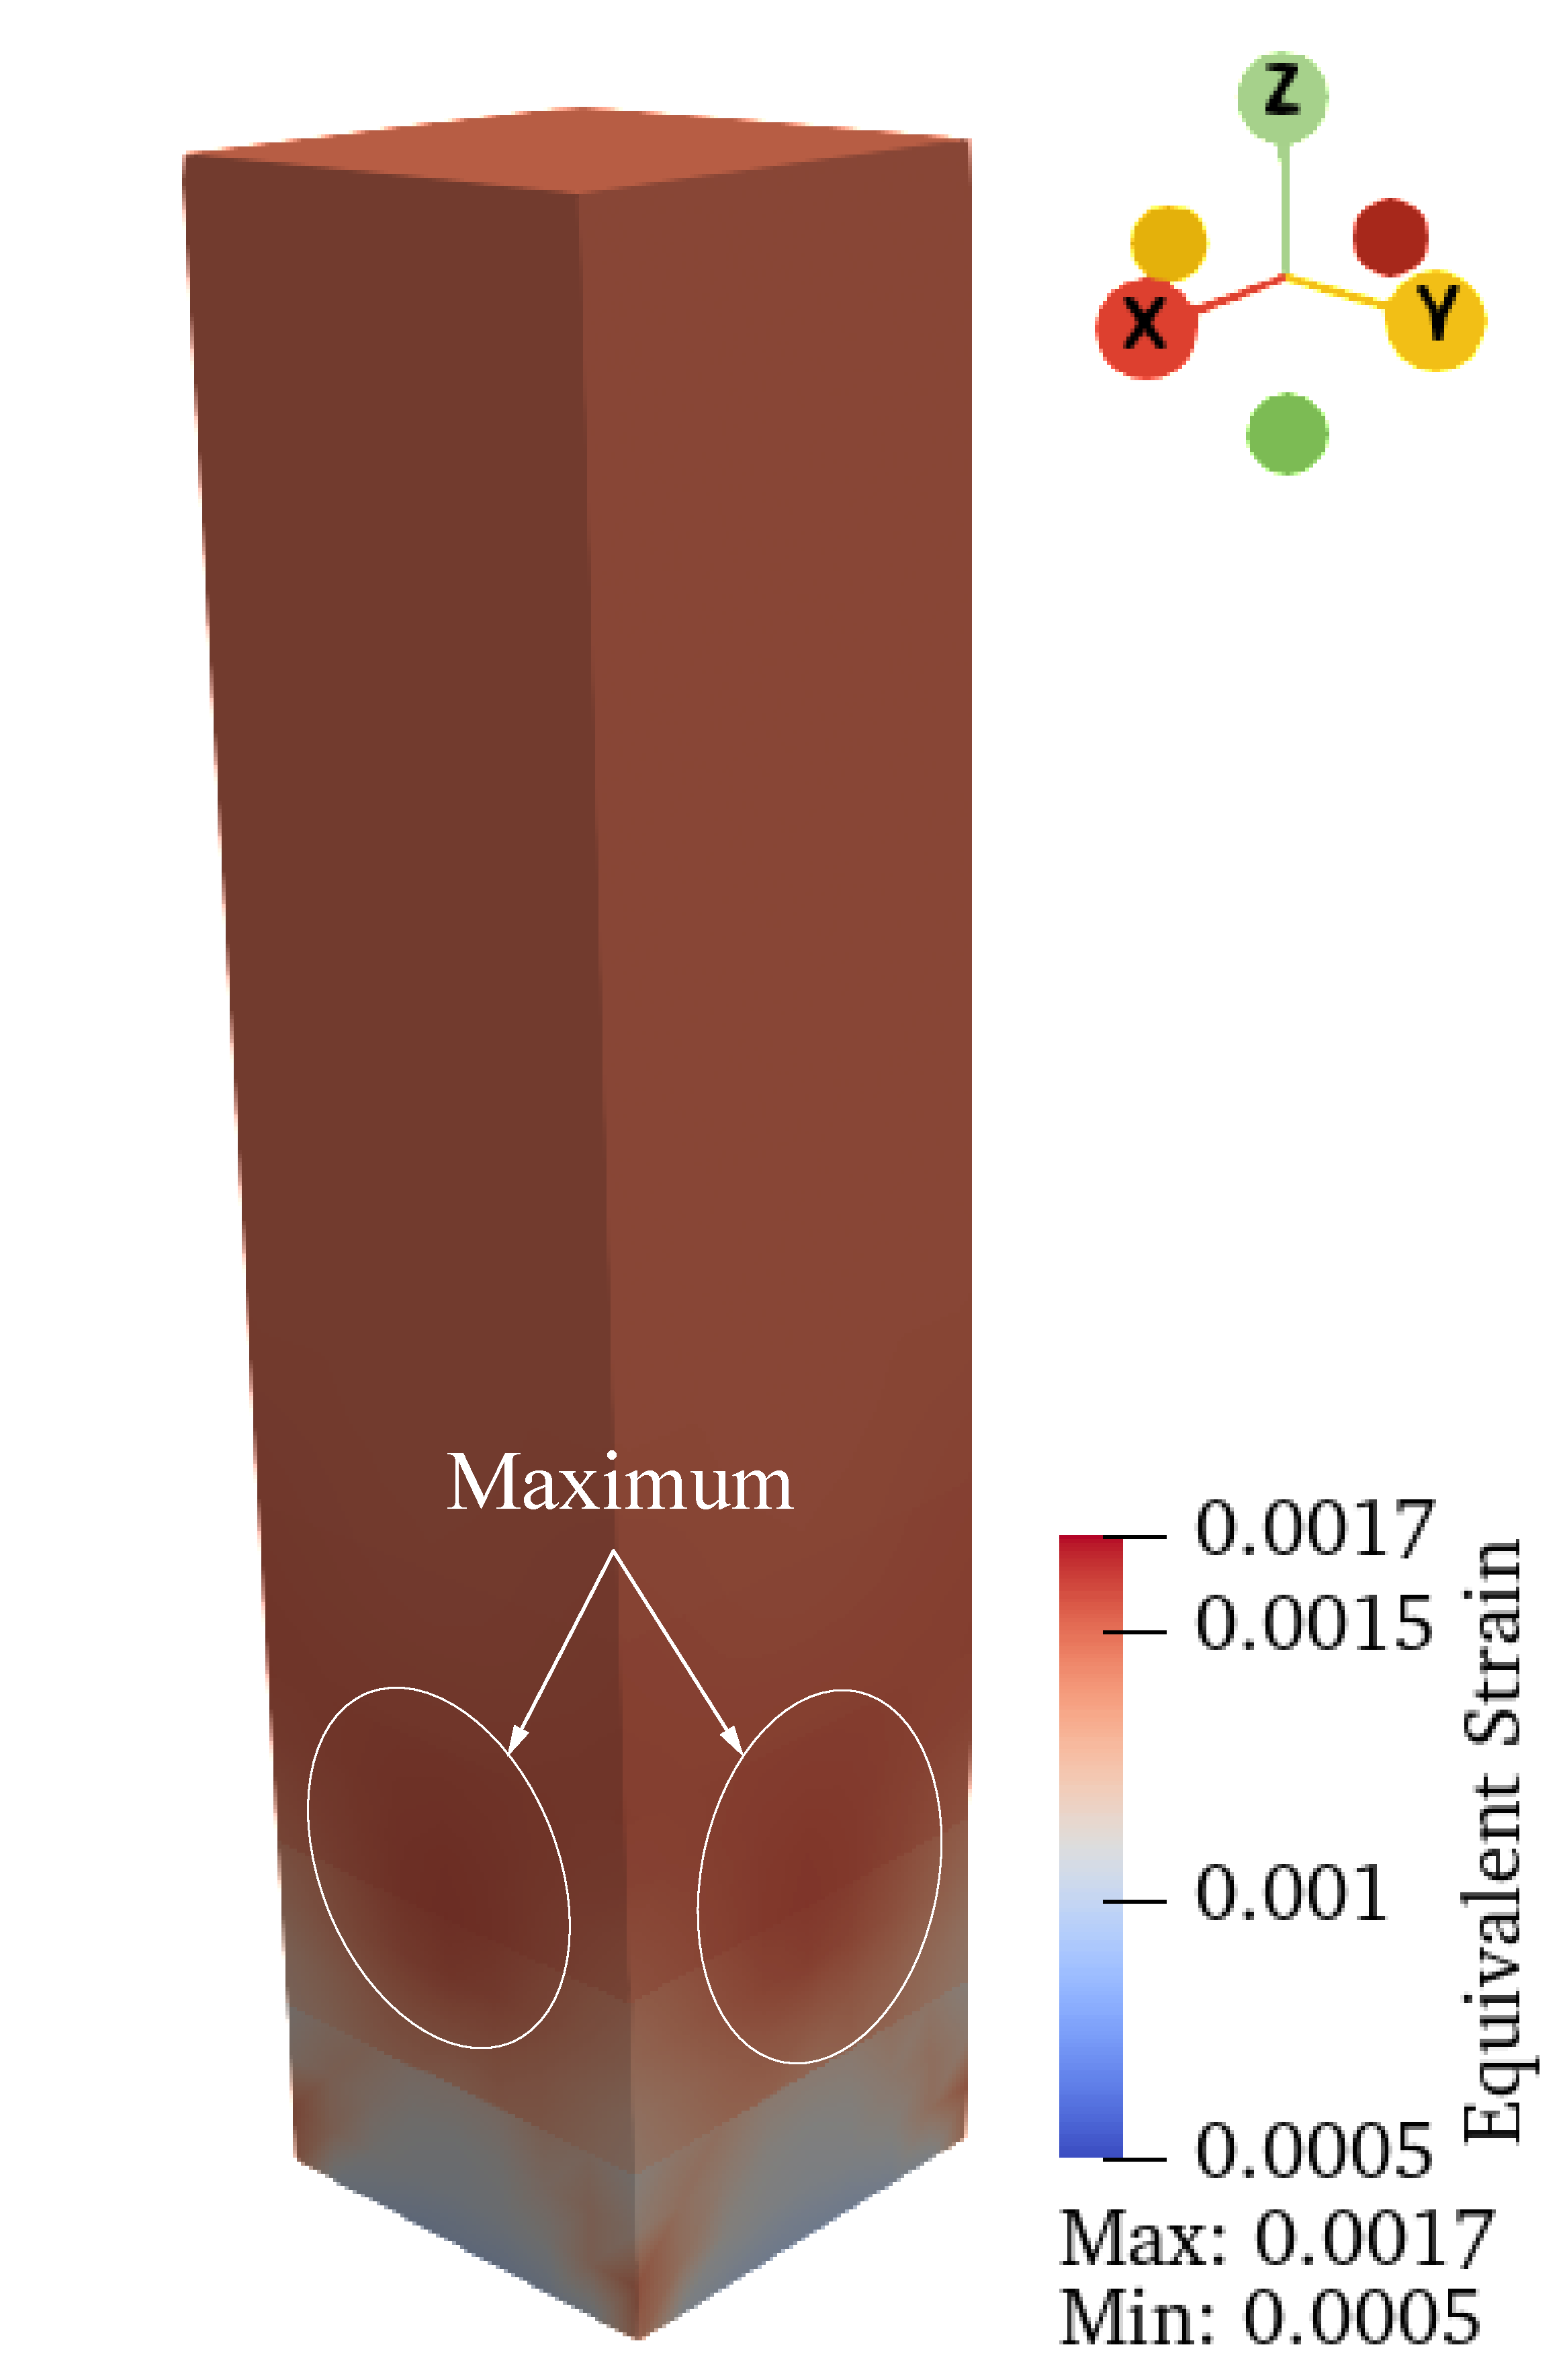
\includegraphics[width=\textwidth]{equivalent_strain1.pdf}
        \caption{Equivalent strain}
    \end{subfigure}
    \begin{subfigure}{0.27\textwidth}
        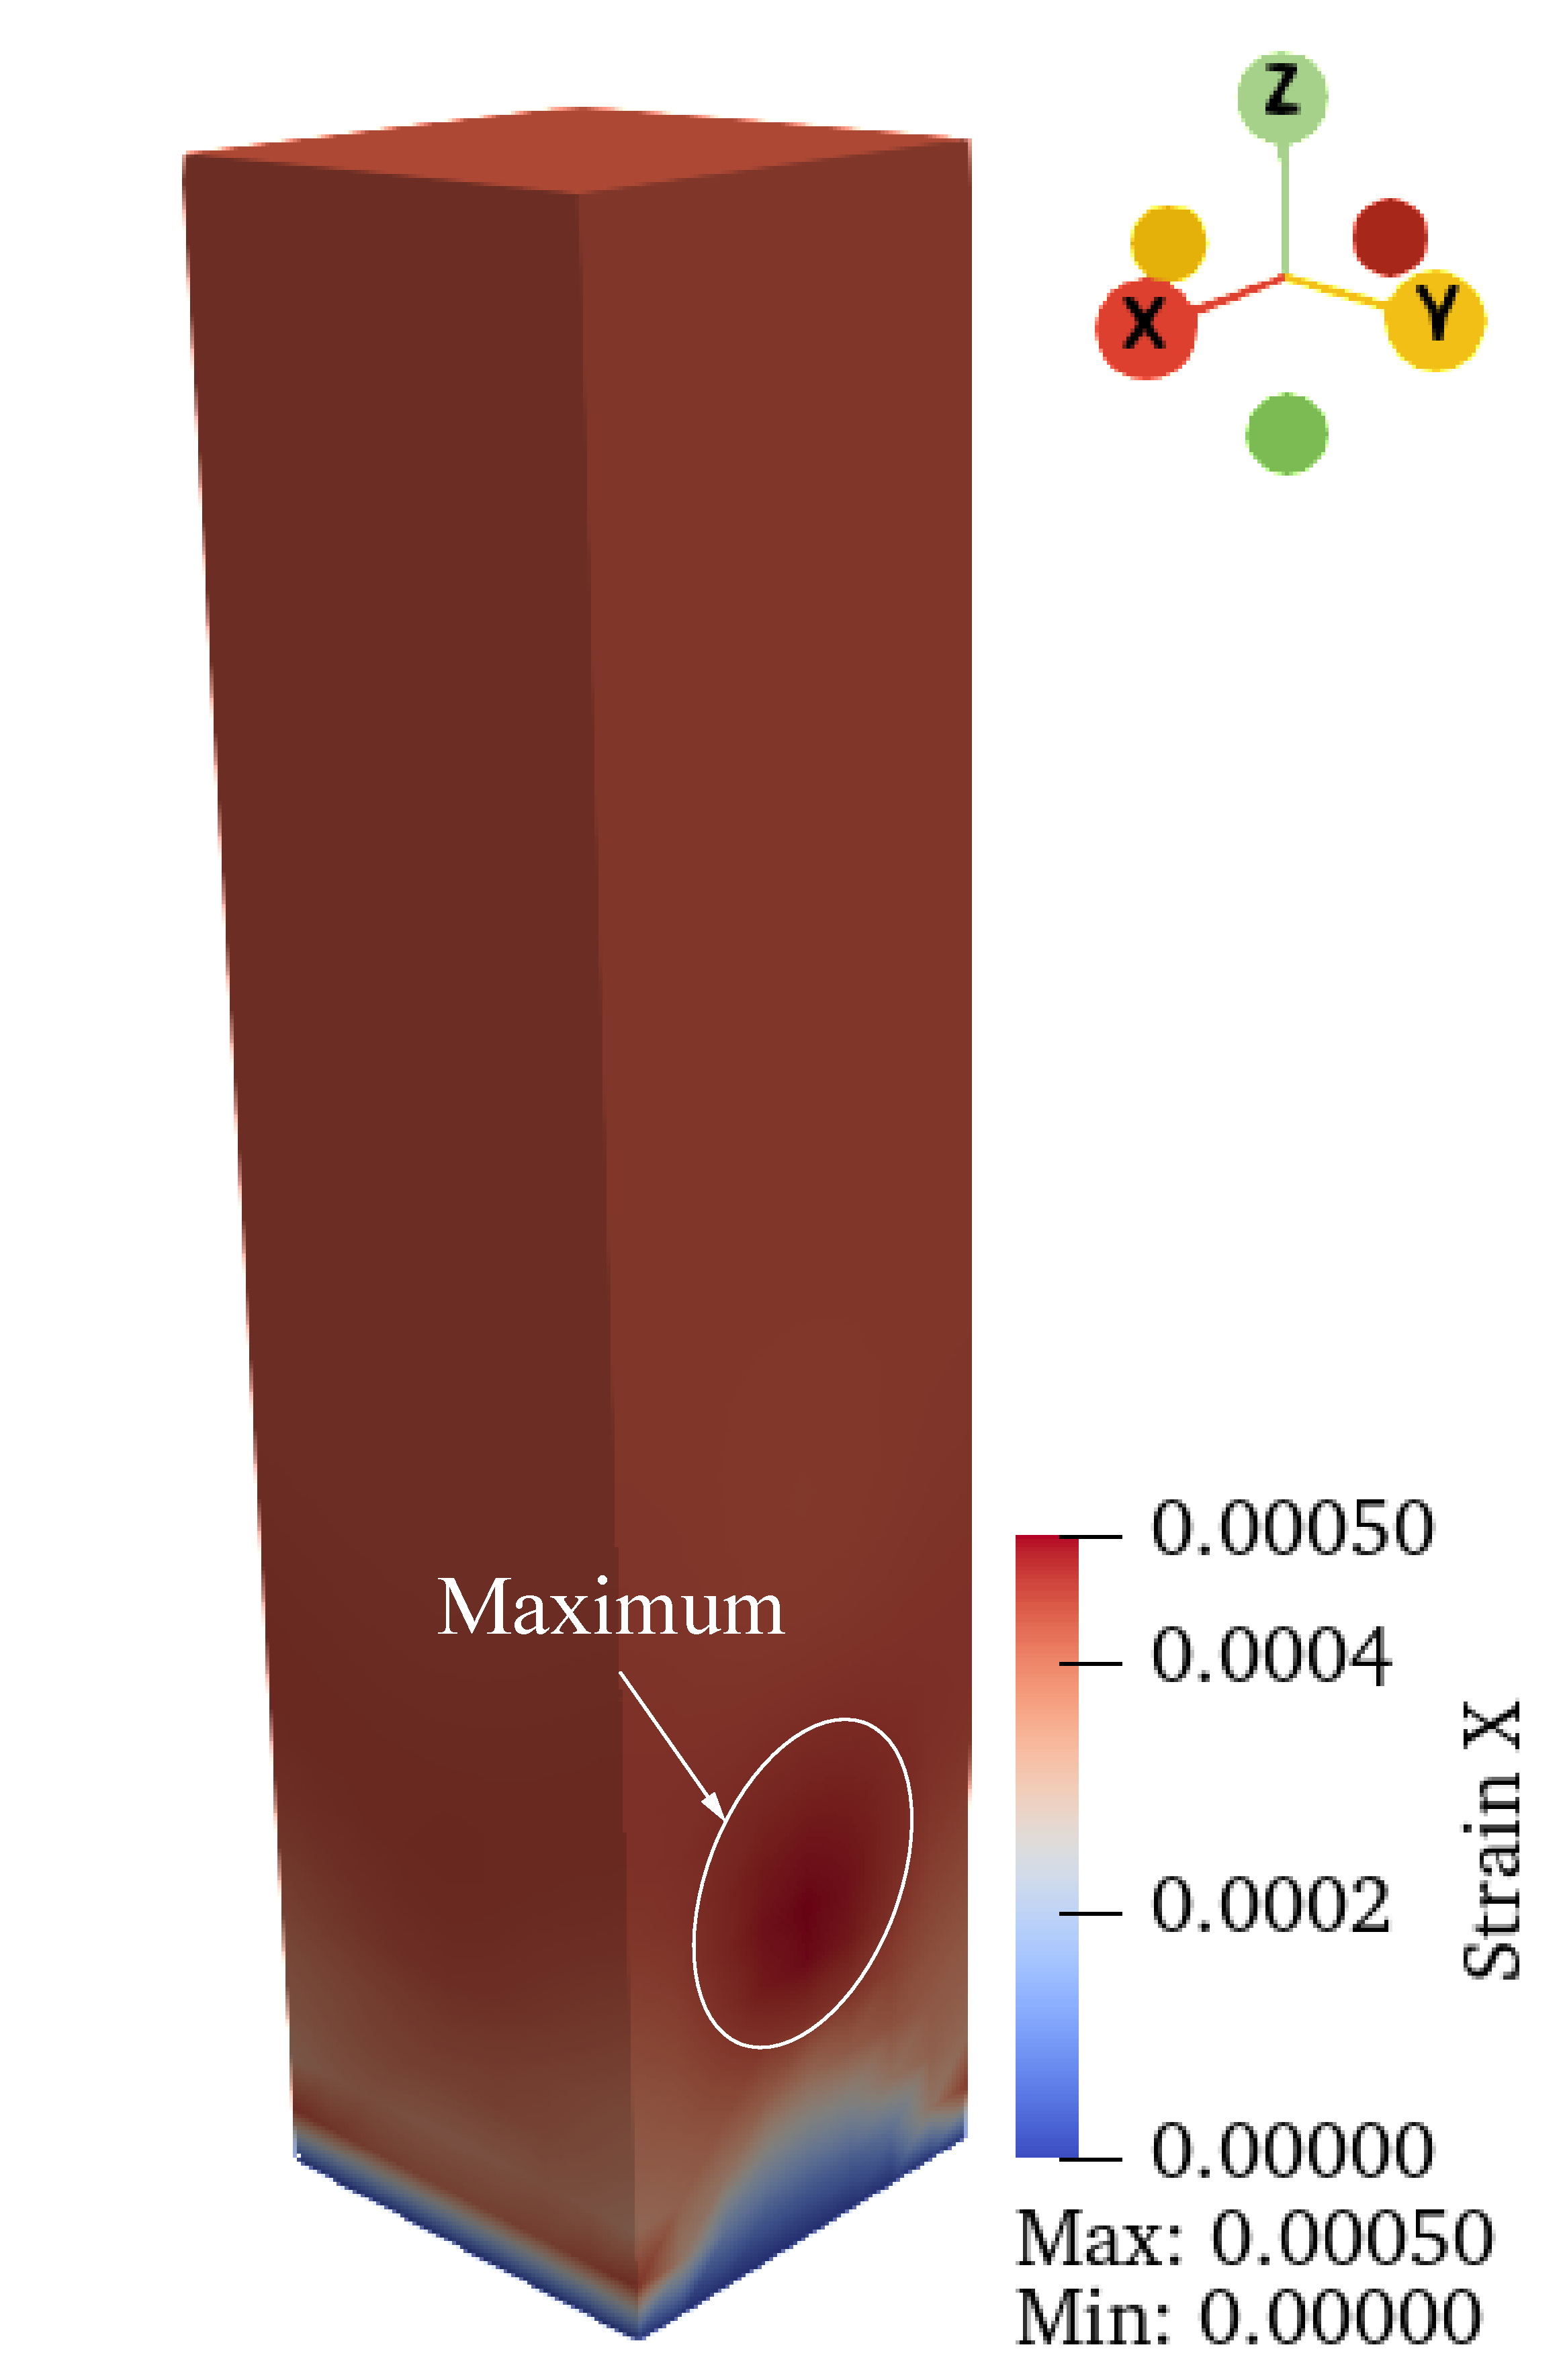
\includegraphics[width=\textwidth]{strain_x1.pdf}
        \caption{Strain in $x$ direction}
    \end{subfigure}

    \caption{Numerical results: observed equivalent strains, and directional strain distributions.}
    \label{fig:comparison_across_layers}
\end{figure}

\section{Results from Physics-Informed Graph Neural Networks}

\subsection{Incremental-Iterative Framework and Graph-Based Network Architecture}
\label{subsec:iterative_framework}

The procedure illustrated in Fig.~\ref{fig:flowchart} outlines the incremental-iterative framework used to capture the load-displacement response of a layered column. The simulation begins with the first load step applied to the top layer. For each step, random spatial coordinates are generated within the active layer, normalized, and provided as input to the neural network model. The network predicts the displacement and stress fields, which are subsequently denormalized to recover their physical scales. From the predicted stress field, the bottom stress of the current layer is extracted and applied as the boundary condition for the layer immediately below, ensuring consistent load transfer throughout the column. Once stresses across all layers are determined, the Mazars damage model is applied to evaluate the damage variable at each spatial point, accounting for stiffness degradation and microcracking. The load is then incremented, and the procedure is repeated up to failure. This framework captures both the mechanical response and the progressive damage evolution across successive loading stages. 

\begin{figure}[t]
    \centering
    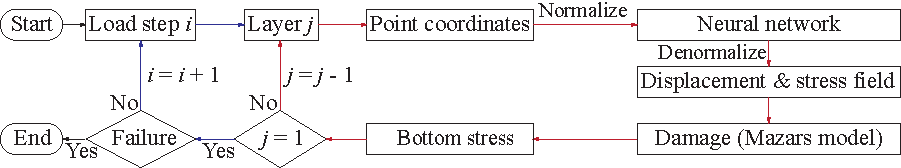
\includegraphics[width=0.75\textwidth]{flowchart.pdf}
    \captionsetup{justification=centering}
    \caption{Incremental-iterative framework for predicting the load-displacement response of a layered 3DPC column using physics-informed graph neural networks.}
    \label{fig:flowchart}
\end{figure}

Unlike conventional supervised machine-learning models, the present PINN is formulated as an alternative field solver for contact and solid mechanics. The column geometry and material properties are prescribed from the experimental validation case, while the graph contains 2,048 normalized spatial collocation points. Their coordinates, $x$, $y$, and $z$, are used as node features because they define the three-dimensional domain and are required to evaluate spatial derivatives, enforce equilibrium, and apply the boundary and contact conditions. The $z$-coordinate represents the loading direction and layerwise load transfer, whereas $x$ and $y$ describe lateral deformation and tangential variation along the interfaces. The network predicts three displacement and six stress components throughout the domain. Conventional feature inclusion or exclusion was not applied because removing a coordinate would reduce the physical dimensionality and prevent prediction of the complete three-dimensional response. Coordinate significance is instead evaluated through the node-feature-importance analysis in Section~\ref{subsubsec:node_feature_importance}.

The 3DPC column in Fig.~\ref{fig:compression_across_layers} is symmetric about both the $x$- and $y$-axes; therefore, only one-quarter of the cross-section is modeled to improve computational efficiency. As shown in Fig.~\ref{fig:bcs}, a compressive stress $\sigma_{zz} = -p$ is applied to the top surface, while $\sigma_{zx}$ and $\sigma_{zy}$ are set to zero. On the negative $x$- and $y$-faces, the normal displacements $u_{xx}$ and $u_{yy}$ are constrained to zero by symmetry. The positive $x$- and $y$-faces are traction-free, with $\sigma_{xx}$, $\sigma_{yy}$, $\sigma_{xy}$, $\sigma_{xz}$, $\sigma_{yx}$, and $\sigma_{yz}$ set to zero. At the interlayer interfaces, the contact conditions follow Section~\ref{subsec:node_to_surface}, with $t_x = t_y = 0$, $g_\text{n} \geq 0$, $p_\text{n} \leq 0$, and $p_\text{n} g_\text{n} = 0$. The complementarity condition is equivalently expressed using the Fischer--Burmeister function~\citep{fischer_special_1992} as:
\begin{align}
    g_\text{n} - p_\text{n} - \sqrt{g_\text{n}^2 + p_\text{n}^2} = 0 %\, .
\end{align}
During training, the governing equations and the prescribed boundary and contact conditions are evaluated at the corresponding collocation points and imposed as residual terms in the physics-informed loss function. Minimizing these residuals constrains the predicted displacement and stress fields to satisfy the mechanical equilibrium and boundary-value problem.

\begin{figure}[t]
    \centering
    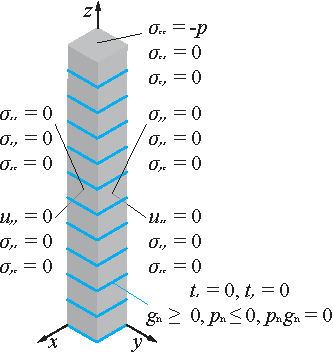
\includegraphics[width=0.4\textwidth]{bcs.pdf}
    \caption{Boundary conditions of the 3DPC column within the PINN framework.}
    \label{fig:bcs}
\end{figure}

The choice of network architecture is critical to physics-informed modeling. Conventional PINNs commonly use fully connected MLPs that process each coordinate independently and therefore do not explicitly capture spatial relationships. To address this limitation, the present study adopts a residual GraphSAGE architecture in which each point is connected to its eight nearest neighbors. As shown in Fig.~\ref{fig:ResGraphSAGE}, the network maps the three input coordinates to a hidden feature space through a linear projection, followed by two SAGEConv layers with layer normalization and Gaussian error linear unit (GELU) activation. A residual pathway preserves geometric information and mitigates over-smoothing, while a final linear layer maps the hidden representation to nine displacement and stress outputs. This architecture incorporates local geometric and topological information while maintaining computational efficiency.

\begin{figure}[t]
    \centering
    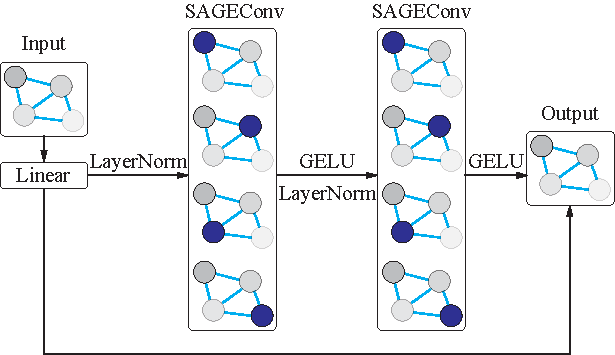
\includegraphics[width=0.5\textwidth]{ResGraphSAGE.pdf}
    \caption{GraphSAGE-based residual network for displacement and stress prediction.}
    \label{fig:ResGraphSAGE}
\end{figure}

\subsection{Model Evaluation and Comparative Performance Analysis}

Validation followed a two-stage hierarchy. The FEM was first validated against the experimental load-displacement response of the eleven-layer column, establishing a reference solution for the investigated configuration. The MLP and residual GNN were then evaluated against the validated FEM because the experiment provides the global response, whereas the FEM provides the spatial displacement and stress fields required for field-level comparison. This procedure evaluates whether the PINNs reproduce the reference mechanical solution, but does not constitute direct experimental validation of the PINNs.

Both architectures map the three normalized spatial coordinates $(x,y,z)$ to nine outputs comprising three displacement and six stress components. The MLP contains five fully connected hidden layers with $\tanh$ activations, followed by a linear output layer, consistent with~\citet{sahin_solving_2024} (Fig.~\ref{fig:MLP}). The residual GNN consists of a linear input projection, two SAGEConv layers with layer normalization and GELU activations, a residual connection, and a linear output head. Four hidden dimensions ranging from 2 to 8 were examined, corresponding to 59 -- 401 trainable parameters for the MLP and 69 -- 225 for the GNN, as summarized in Table~\ref{tab:archetecture}. The GNN depth was limited to two convolutional layers to reduce over-smoothing. Both models were trained using the same equilibrium and boundary/contact residual losses without labeled data.

\begin{figure}[t]
    \centering
    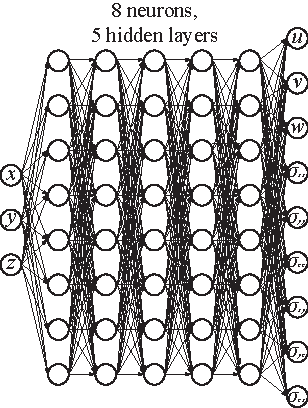
\includegraphics[width=0.3\textwidth]{mlp.pdf}
    \caption{Architecture of the five-layer MLP used for displacement and stress prediction in the 3DPC column.}
    \label{fig:MLP}
\end{figure}

\begin{table}[t]
    \centering
    \footnotesize
    \caption{Architectures of MLPs and GNNs.}
    \begin{tabular}{
        >{\centering\arraybackslash}p{1.5cm} 
        >{\centering\arraybackslash}p{4.5cm} 
        >{\centering\arraybackslash}p{4.5cm}}
        \toprule
        Cases & MLPs (No. of parameters) & GNNs (No. of parameters) \\
        \midrule
        Case 1 & 8 neurons, 5 layers (401) & 8 dimensions, 2 layers (225) \\
        Case 2 & 4 neurons, 5 layers (141) & 4 dimensions, 2 layers (139) \\
        Case 3 & 3 neurons, 5 layers (96) & 3 dimensions, 2 layers (90) \\
        Case 4 & 2 neurons, 5 layers (59) & 2 dimensions, 2 layers (69) \\
        \bottomrule
    \end{tabular}
    \label{tab:archetecture}
\end{table}

\begin{figure}[t]
    \centering
    \begin{subfigure}{0.49\textwidth}
        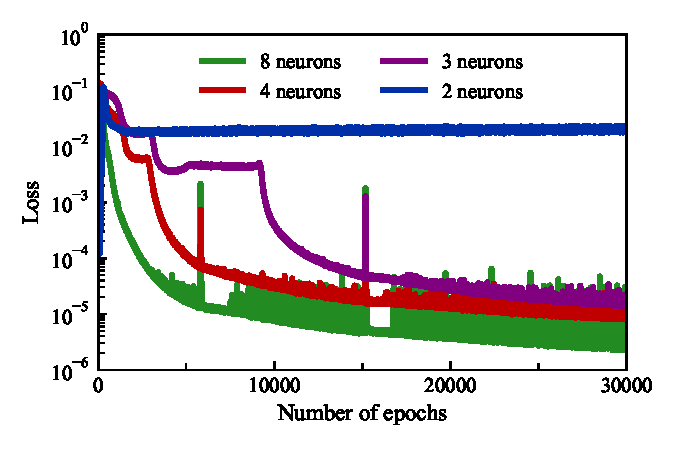
\includegraphics[width=\textwidth]{training_process_mlp_pde.pdf}
        \caption{PDE residual loss of MLPs.}
    \end{subfigure}
    \hfill
    \begin{subfigure}{0.49\textwidth}
        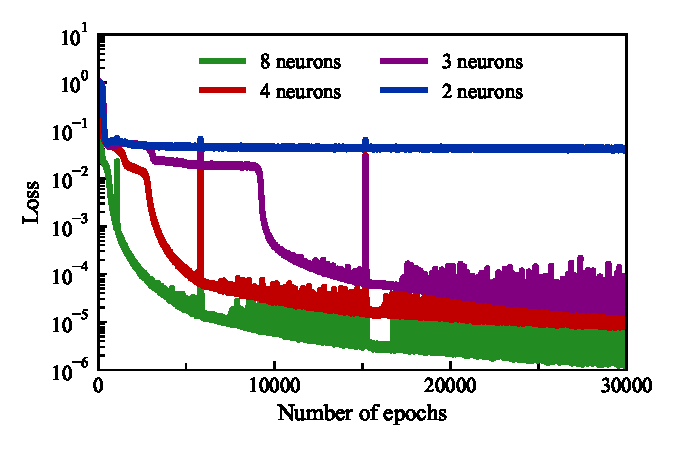
\includegraphics[width=\textwidth]{training_process_mlp_bcs.pdf}
        \caption{Boundary-condition loss of MLPs.}
    \end{subfigure}

    \vspace{0.5em}

    \begin{subfigure}{0.49\textwidth}
        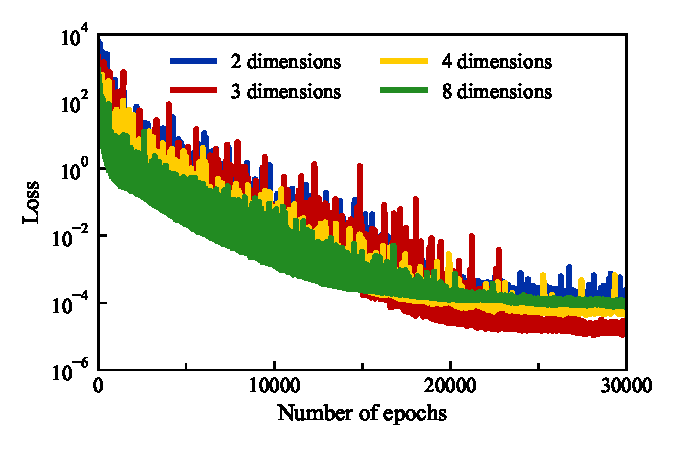
\includegraphics[width=\textwidth]{training_process_graph_pde.pdf}
        \caption{PDE residual loss of GNNs.}
    \end{subfigure}
    \hfill
    \begin{subfigure}{0.49\textwidth}
        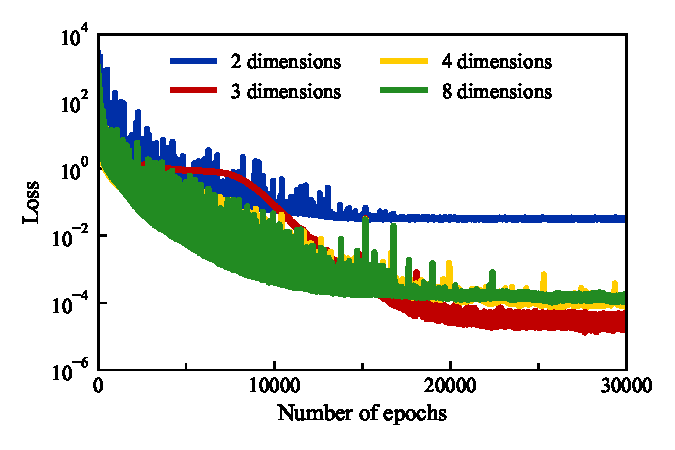
\includegraphics[width=\textwidth]{training_process_graph_bcs.pdf}
        \caption{Boundary-condition loss of GNNs}
    \end{subfigure}

    \captionsetup{justification=centering}
    \caption{PDE and boundary-condition loss histories of the tested MLPs and GNNs.}
    \label{fig:traning_process}
\end{figure}

Both MLP and GNN models were trained under identical settings on a system with a 12th Gen Intel\textsuperscript{\textregistered} Core\texttrademark~i7-12700 CPU and an NVIDIA T1000 GPU. The Adam optimizer was used for 30{,}000 epochs with a learning rate of 0.001, while all other settings followed the PyTorch defaults~\citep{paszke_pytorch_2019}. The total loss combined the partial differential equation (PDE) residual in Eqn.~(\ref{eq:governing_equation}) with the displacement and stress boundary-condition residuals in Fig.~\ref{fig:bcs}. As shown in Fig.~\ref{fig:traning_process}, the MLP losses decreased steadily after approximately 10{,}000 epochs, with the four-neuron model providing the best balance of accuracy, stability, and parameter efficiency. The GNN losses decreased more slowly during the first 20{,}000 epochs, but the three-dimension model ultimately achieved the lowest loss, whereas higher-dimensional variants produced larger residuals. Fig.~\ref{fig:total_loss} compares the selected models, showing that the 90-parameter GNN achieved a loss comparable to the 141-parameter MLP by exploiting spatial connectivity.

\begin{figure}[t]
    \centering
    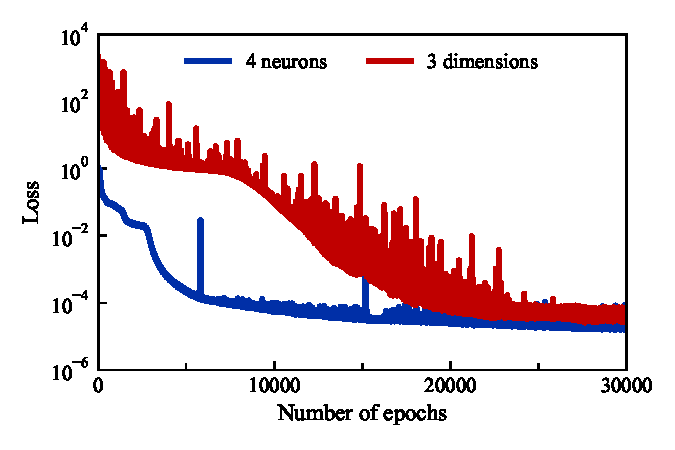
\includegraphics[width=0.57\textwidth]{training_process_total_loss.pdf}
    \captionsetup{justification=centering}
    \caption{Total loss histories of the selected MLP and GNN models.}
    \label{fig:total_loss}
\end{figure}

As shown in Fig.~\ref{fig:response_comparison}, both models reproduced the load-displacement response of the 3DPC column with high accuracy. The load RMSEs were nearly identical, as expected under load-controlled conditions. However, the GNN achieved a lower displacement RMSE of $0.002 \, \text{mm}$, compared with $0.003 \, \text{mm}$ for the MLP, while using 90 rather than 141 trainable parameters, representing a 36.2\% reduction. These results indicate that the GNN can achieve comparable or improved predictive accuracy with greater parameter efficiency by explicitly leveraging spatial connectivity among points.

\begin{figure}[t]
    \centering
    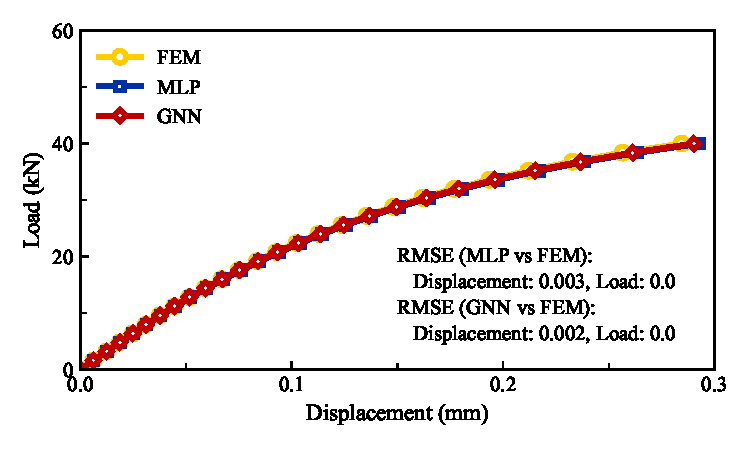
\includegraphics[width=0.6\textwidth]{response_comparison.pdf}
    \captionsetup{justification=centering}
    \caption{FEM, MLP, and GNN load-displacement responses and displacement RMSEs.}
    \label{fig:response_comparison}
\end{figure}

\subsection{Explanation of Graph Neural Network}

\subsubsection{Theoretical Advantage of GNN over MLP}

To interpret the benefit of graph connectivity in physics-informed learning, the benign generalization framework~\citep{cao_benign_2022, huang_quantifying_2025} is adopted. The signal-to-noise ratio (SNR) measures the magnitude of the meaningful structural-response signal relative to random variations introduced by coordinate sampling and numerical approximation:

\begin{equation}
    \mathrm{SNR} =
    \frac{\|\boldsymbol{\mu}\|_2}
    {\sigma_{\text{p}}\sqrt{d_{\text{f}}}},
\end{equation}
where $\|\boldsymbol{\mu}\|_2$ is the signal magnitude, $\sigma_{\text{p}}$ is the noise level, and $d_{\text{f}}$ is the feature dimension.

The analysis assumes a signal-plus-noise representation, a polynomial activation exponent $q>2$, sufficient training samples, and largely uncorrelated noise among neighboring nodes. Under these assumptions, an MLP requires $n_{\text{ts}}\mathrm{SNR}^{q}=\tilde{\Omega}(1)$ for low test error. Neighborhood aggregation increases the effective SNR of a GNN as
\begin{equation}
    \mathrm{SNR}_{\text{GNN}}
    =
    \mathrm{SNR}_{\text{MLP}}
    D^{\frac{q-2}{2q}},
\end{equation}
where $D$ is the expected node degree. The corresponding minimum SNRs are
\begin{equation}
    \mathrm{SNR}_{\text{MLP,min}}
    =
    (C/n_{\text{ts}})^{1/q},
    \qquad
    \mathrm{SNR}_{\text{GNN,min}}
    =
    (C/n_{\text{ts}})^{1/q}
    D^{-\frac{q-2}{2q}},
\end{equation}
and their ratio is
\begin{equation}
    \frac{\mathrm{SNR}_{\text{MLP,min}}}
    {\mathrm{SNR}_{\text{GNN,min}}}
    =
    D^{\frac{q-2}{2q}}.
    \label{eq:snr_advantage}
\end{equation}
The present graph contains $n_{\text{ts}}=2{,}048$ nodes and $8{,}192$ edges, with an average degree of $D=8.0$. Because the original theory was developed for classification with polynomial activations, its application to the present regression-based PINN with GELU is interpretive; $q=3$ is adopted as a heuristic approximation. Substitution into Eqn.~(\ref{eq:snr_advantage}) gives $D^{1/6}\approx1.4$. Thus, the estimated minimum SNR required by the GNN is approximately 71\% of that required by the MLP, or about 29\% lower. For the same signal strength and sample size, this corresponds to tolerance of approximately 1.4 times greater noise standard deviation, or nearly twice the noise variance. The result suggests improved robustness and potential data efficiency, but does not constitute an empirical guarantee.

\subsubsection{Node Feature Importance}
\label{subsubsec:node_feature_importance}

The explanation of GNNs can be examined using node feature importance. This metric is obtained by generating a node mask that quantifies the relative contribution of each input feature to the model's predictions. For each node, the mask values are averaged and normalized, and global statistics are then computed by aggregating across all nodes. This process yields an interpretable measure of how the GNN leverages spatial coordinates to predict displacements and stresses.

Fig.~\ref{fig:feature_importance} presents the normalized feature importance for the top boundary, bottom boundary, left boundary, and interior nodes. At the loaded top surface, the $z$-coordinate is most influential ($\mu=0.374$), consistent with compression and load transfer along the column axis. At the bottom load-transfer interface, the $x$- and $y$-coordinates each have an importance of approximately 0.500, while the $z$-coordinate is negligible because it is constant on this plane. The tangential coordinates therefore identify spatial variations associated with lateral deformation and the normal-contact and zero-tangential-traction conditions. On the left boundary, the $x$- and $z$-coordinates dominate, whereas the constant $y$-coordinate has near-zero importance, reflecting the lateral boundary conditions and axial variation. Within the column interior, all coordinates contribute, although $z$ remains slightly more influential ($\mu=0.358$), consistent with vertical stress transmission through the printed layers. Overall, the learned feature importance follows the geometry and mechanical boundary conditions of the investigated column.

\begin{figure}[t]
    \centering
    \begin{subfigure}{0.49\textwidth}
        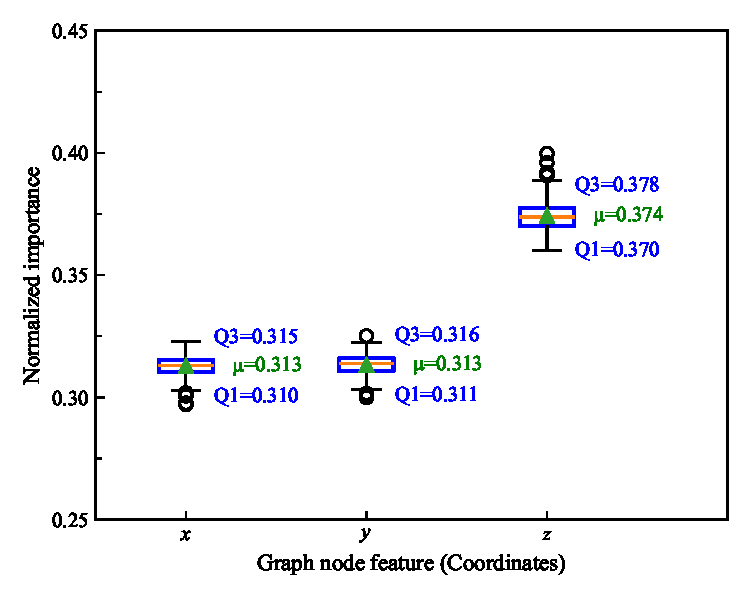
\includegraphics[width=\textwidth]{fi_box_plot_top.pdf}
        \caption{Top boundary points.}
    \end{subfigure}
    \hfill
    \begin{subfigure}{0.49\textwidth}
        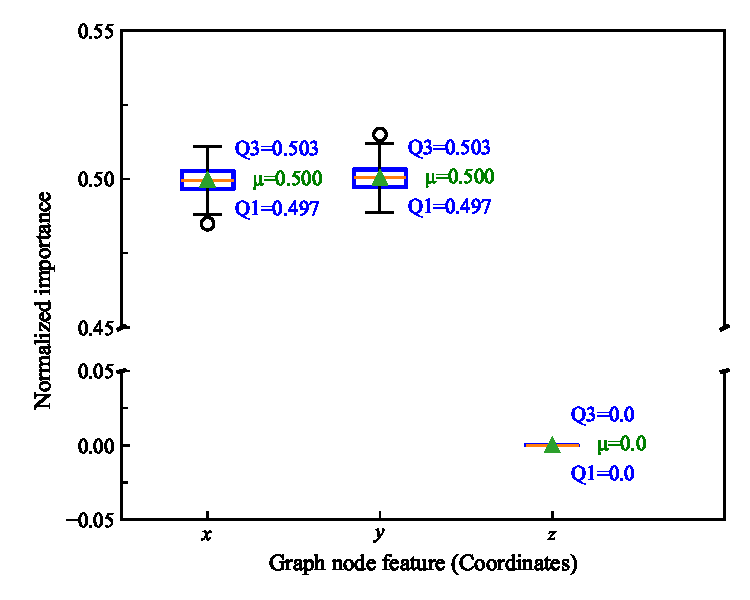
\includegraphics[width=\textwidth]{fi_box_plot_bottom.pdf}
        \caption{Bottom boundary points.}
    \end{subfigure}

    \vspace{0.5em}

    \begin{subfigure}{0.49\textwidth}
        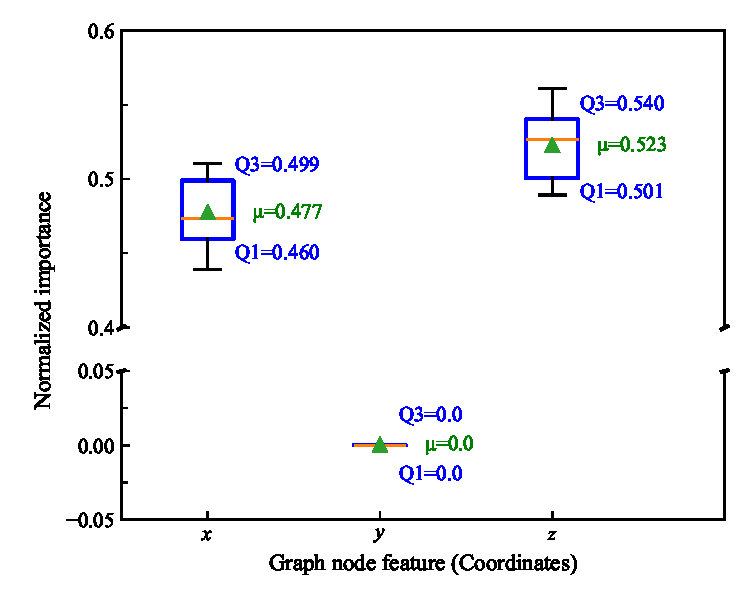
\includegraphics[width=\textwidth]{fi_box_plot_left.pdf}
        \caption{Left boundary points.}
    \end{subfigure}
    \hfill
    \begin{subfigure}{0.49\textwidth}
        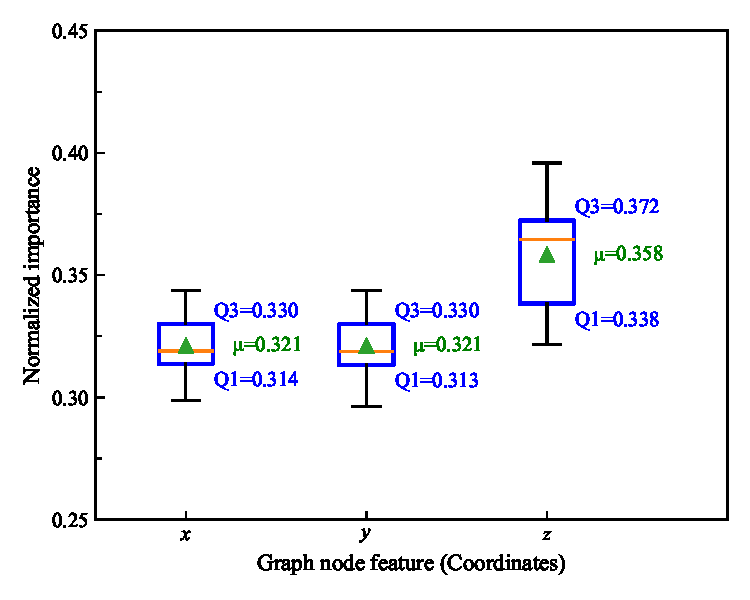
\includegraphics[width=\textwidth]{fi_box_plot_inside.pdf}
        \caption{Interior points.}
    \end{subfigure}

    \caption{Coordinate importance for different node groups under axial compression.}
    \label{fig:feature_importance}
\end{figure}

Fig.~\ref{fig:subgraph} presents the explanatory subgraph for node 8 on the loaded top surface. The nine nodes were generated by Latin hypercube sampling, and edges with importance scores below 0.5 were removed. Nodes 1, 2, and 6 provide the strongest information to node 8, while node 8 strongly influences nodes 3, 5, and 6. These connections form local message-passing pathways associated with axial load introduction, stress transfer, and displacement compatibility near the symmetry boundaries. Because the target node is located on the top surface, this subgraph primarily represents the load-introduction region. It does not directly demonstrate attention to the lower strain-localization zone identified by the FEM or to the interlayer contact regions, which would require subgraphs centered on those locations.

\begin{figure}[t]
    \centering
    \begin{subfigure}[b]{0.3\textwidth}
        \centering
        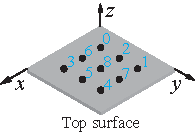
\includegraphics[width=0.85\textwidth]{top_surface.pdf}
        \captionsetup{margin={0em, -2em}, justification=centering}
        \caption{Node indices on the top surface.}
    \end{subfigure}
    \hfill
    \begin{subfigure}[b]{0.65\textwidth}
        \centering
        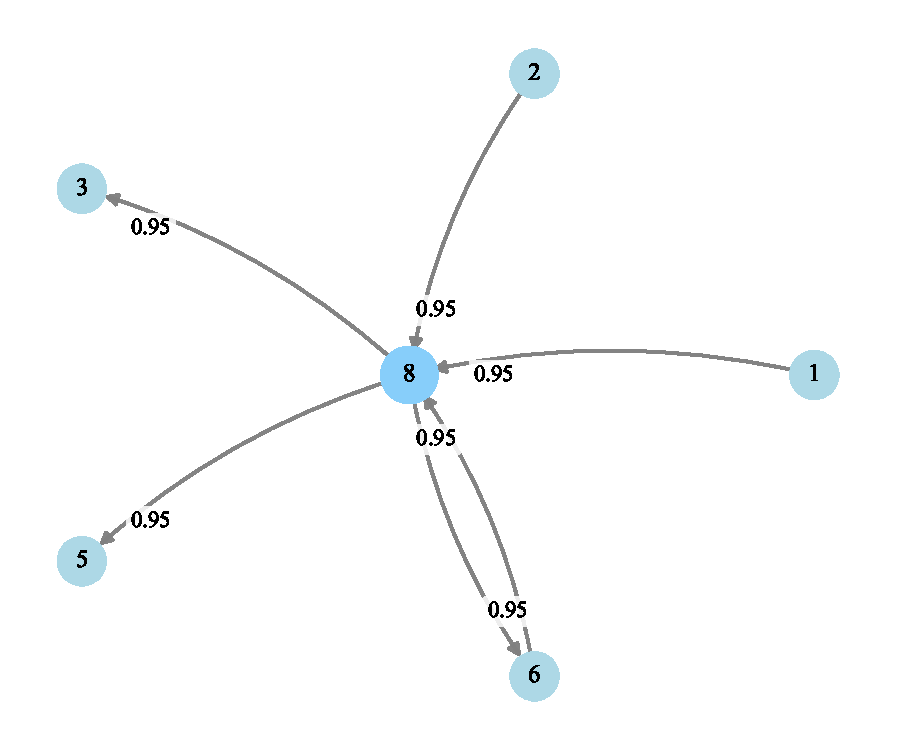
\includegraphics[width=\textwidth]{subgraph_node8.pdf}
        \caption{Explanatory subgraph for node 8 on the top surface.}
    \end{subfigure}

    \caption{Explanatory subgraph for node 8 on the loaded top surface after applying a threshold.}
    \label{fig:subgraph}
\end{figure}

\section{Implications, Limitations, and Future Work}

\subsection{Theoretical and Practical Implications}

The results suggest that graph-based neighborhood aggregation provides a physically meaningful spatial inductive bias, improving the robustness and interpretability of mechanics-informed field prediction. Once validated across a broader design space, the framework could support preliminary comparison of layer configurations, interface properties, and loading directions; identify critical interfaces and high-response regions from predicted displacement and stress fields; and prioritize cases requiring detailed FEM analysis or experimental testing. These decision-support applications remain prospective because the present study considers only one structural configuration.

\subsection{Limitations and Future Work}

The present study considers a single eleven-layer column with fixed geometry, material properties, printing direction, and loading. The non-regularized Mazars model may introduce strain localization and mesh sensitivity. The penalty contact formulation is stiffness-dependent, and the idealized interfaces neglect cohesive fracture, printing-induced heterogeneity, and interlayer variability. The PINNs were evaluated against FEM fields rather than full-field experiments. Moreover, the benign generalization result remains interpretive because the underlying theory assumes a different learning setting. Future work will address broader experimental validation, regularized damage and cohesive-interface models, additional geometries and load cases, computational benchmarking, and integration into preliminary design workflows.

\section{Conclusions}

This study developed an open-source computational framework combining a contact- and damage-based FEM with physics-informed neural networks to predict the compressive behavior of multilayer 3DPC. The FEM was first validated against an experimental column, and the MLP and residual GNN were subsequently evaluated as alternative field solvers against the FEM response. The principal findings are summarized as follows:

\begin{enumerate}
    \item The FEM incorporating node-to-surface contact and the Mazars damage model reproduced the overall experimental load-displacement response and captured the development of nonlinear stiffness degradation. The predicted peak load was 19.5\% lower than the experimental value, while the corresponding displacement error was 7.7\%. The remaining discrepancy indicates that further calibration of the constitutive and interlayer formulations is required.

    \item Both physics-informed architectures closely reproduced the FEM response for the investigated column. The residual GNN achieved a displacement RMSE of 0.002~mm using 90 trainable parameters, compared with 0.003~mm and 141 parameters for the MLP. These results indicate that incorporating local spatial connectivity can improve parameter efficiency while maintaining comparable or slightly improved prediction accuracy.

    \item The benign generalization analysis produced an MLP-to-GNN minimum-SNR ratio of approximately 1.4, suggesting that graph-based neighborhood aggregation may improve robustness to input variations. The feature-importance analysis identified the $z$-coordinate as the dominant feature near the loaded surface and within the column interior, while the subgraph analysis revealed message-passing pathways consistent with the imposed boundary conditions and load-transfer mechanism.
\end{enumerate}

\section*{Acknowledgements}

This work was supported by the US Department of Housing and Urban Development (HUD) under Grant Project FAIN\#B-24-CP-WI-2320 to Marquette University's Opus College of Engineering, entitled Training Workforce for Infrastructure Construction and Engineering (TWICE) Project.

\section*{Funding}
The authors disclosed receipt of the following financial support for the research, authorship, and/or publication of this article: This work was supported by the US Department of Housing and Urban Development (HUD) under Grant Project FAIN\#B-24-CP-WI-2320 to Marquette University's Opus College of Engineering, entitled Training Workforce for Infrastructure Construction and Engineering (TWICE) Project.

\section*{Declaration of Conflicting Interests}
The authors declared no potential conflicts of interest with respect to the research, authorship, and/or publication of this article.

\section*{Data Availability Statement}
The source code and data supporting the findings of this study are publicly available at \url{https://github.com/ZhangHaoyou/3DPC-FEM-PIGNN}. The repository contains the implementations of the finite element method and the physics-informed neural network models, the configuration files defining the analyzed cases, and the load-displacement data used for validation and model evaluation. These materials are provided to facilitate reproducibility and further research.

\bibliographystyle{SageH}
\bibliography{references}


\end{document}

\endinput
